\documentclass[journal,oneside,a4paper,onecolumn]{IEEEtran}

% Some very useful LaTeX packages include:
% (uncomment the ones you want to load)

% *** CITATION PACKAGES ***
%
\usepackage{cite}
% cite.sty was written by Donald Arseneau
% V1.6 and later of IEEEtran pre-defines the format of the cite.sty package
% \cite{} output to follow that of IEEE. Loading the cite package will
% result in citation numbers being automatically sorted and properly
% "compressed/ranged". e.g., [1], [9], [2], [7], [5], [6] without using
% cite.sty will become [1], [2], [5]--[7], [9] using cite.sty. cite.sty's
% \cite will automatically add leading space, if needed. Use cite.sty's
% noadjust option (cite.sty V3.8 and later) if you want to turn this off.
% cite.sty is already installed on most LaTeX systems. Be sure and use
% version 4.0 (2003-05-27) and later if using hyperref.sty. cite.sty does
% not currently provide for hyperlinked citations.
% The latest version can be obtained at:
% http://www.ctan.org/tex-archive/macros/latex/contrib/cite/
% The documentation is contained in the cite.sty file itself.


% *** GRAPHICS RELATED PACKAGES ***
%
  \usepackage{graphicx}
  \graphicspath{{figs/}}
  \DeclareGraphicsExtensions{.pdf,.png}
  \usepackage{color}

% *** MATH PACKAGES ***
%
\usepackage[cmex10]{amsmath}
% A popular package from the American Mathematical Society that provides
% many useful and powerful commands for dealing with mathematics. If using
% it, be sure to load this package with the cmex10 option to ensure that
% only type 1 fonts will utilized at all point sizes. Without this option,
% it is possible that some math symbols, particularly those within
% footnotes, will be rendered in bitmap form which will result in a
% document that can not be IEEE Xplore compliant!
%
% Also, note that the amsmath package sets \interdisplaylinepenalty to 10000
% thus preventing page breaks from occurring within multiline equations. Use:
%\interdisplaylinepenalty=2500
% after loading amsmath to restore such page breaks as IEEEtran.cls normally
% does. amsmath.sty is already installed on most LaTeX systems. The latest
% version and documentation can be obtained at:
% http://www.ctan.org/tex-archive/macros/latex/required/amslatex/math/

%\usepackage{amssymb}%............................ AMS Symbol fonts



% *** SPECIALIZED LIST PACKAGES ***
%
%\usepackage{algorithmic}
% algorithmic.sty was written by Peter Williams and Rogerio Brito.
% This package provides an algorithmic environment for describing algorithms.
% You can use the algorithmic environment in-text or within a figure
% environment to provide for a floating algorithm. Do NOT use the algorithm
% floating environment provided by algorithm.sty (by the same authors) or
% algorithm2e.sty (by Christophe Fiorio) as IEEE does not use dedicated
% algorithm float types and packages that provide these will not provide
% correct IEEE style captions. The latest version and documentation of
% algorithmic.sty can be obtained at:
% http://www.ctan.org/tex-archive/macros/latex/contrib/algorithms/
% There is also a support site at:
% http://algorithms.berlios.de/index.html
% Also of interest may be the (relatively newer and more customizable)
% algorithmicx.sty package by Szasz Janos:
% http://www.ctan.org/tex-archive/macros/latex/contrib/algorithmicx/

% *** ALIGNMENT PACKAGES ***
%
\usepackage{array}
% Frank Mittelbach's and David Carlisle's array.sty patches and improves
% the standard LaTeX2e array and tabular environments to provide better
% appearance and additional user controls. As the default LaTeX2e table
% generation code is lacking to the point of almost being broken with
% respect to the quality of the end results, all users are strongly
% advised to use an enhanced (at the very least that provided by array.sty)
% set of table tools. array.sty is already installed on most systems. The
% latest version and documentation can be obtained at:
% http://www.ctan.org/tex-archive/macros/latex/required/tools/


\usepackage{mdwmath}
\usepackage{mdwtab}
% Also highly recommended is Mark Wooding's extremely powerful MDW tools,
% especially mdwmath.sty and mdwtab.sty which are used to format equations
% and tables, respectively. The MDWtools set is already installed on most
% LaTeX systems. The lastest version and documentation is available at:
% http://www.ctan.org/tex-archive/macros/latex/contrib/mdwtools/

% IEEEtran contains the IEEEeqnarray family of commands that can be used to
% generate multiline equations as well as matrices, tables, etc., of high
% quality.

% *** SUBFIGURE PACKAGES ***
% subfig.sty, also written by Steven Douglas Cochran, is the modern
% replacement for subfigure.sty. However, subfig.sty requires and
% automatically loads Axel Sommerfeldt's caption.sty which will override
% IEEEtran.cls handling of captions and this will result in nonIEEE style
% figure/table captions. To prevent this problem, be sure and preload
% caption.sty with its "caption=false" package option. This is will preserve
% IEEEtran.cls handing of captions. Version 1.3 (2005/06/28) and later
% (recommended due to many improvements over 1.2) of subfig.sty supports
% the caption=false option directly:
\usepackage[caption=false,font=footnotesize]{subfig}
%
% The latest version and documentation can be obtained at:
% http://www.ctan.org/tex-archive/macros/latex/contrib/subfig/
% The latest version and documentation of caption.sty can be obtained at:
% http://www.ctan.org/tex-archive/macros/latex/contrib/caption/

%Setting captions to centered (Not IEEE journal standard)
\makeatletter
\long\def\@makecaption#1#2{\ifx\@captype\@IEEEtablestring%
\footnotesize\begin{center}{\normalfont\footnotesize #1}\\
{\normalfont\footnotesize\scshape #2}\end{center}%
\@IEEEtablecaptionsepspace
\else
\@IEEEfigurecaptionsepspace
\setbox\@tempboxa\hbox{\normalfont\footnotesize {#1.}~~ #2}%
\ifdim \wd\@tempboxa >\hsize%
\setbox\@tempboxa\hbox{\normalfont\footnotesize {#1.}~~ }%
\parbox[t]{\hsize}{\normalfont\footnotesize \noindent\unhbox\@tempboxa#2}%
\else
\hbox to\hsize{\normalfont\footnotesize\hfil\box\@tempboxa\hfil}\fi\fi}
\makeatother


% *** FLOAT PACKAGES ***
%
\usepackage{fixltx2e}
% fixltx2e, the successor to the earlier fix2col.sty, was written by
% Frank Mittelbach and David Carlisle. This package corrects a few problems
% in the LaTeX2e kernel, the most notable of which is that in current
% LaTeX2e releases, the ordering of single and double column floats is not
% guaranteed to be preserved. Thus, an unpatched LaTeX2e can allow a
% single column figure to be placed prior to an earlier double column
% figure. The latest version and documentation can be found at:
% http://www.ctan.org/tex-archive/macros/latex/base/

% *** PDF, URL AND HYPERLINK PACKAGES ***
%
\usepackage{url}

\usepackage{sistyle}
    \SIstyle{S-Africa}
    \SIunitspace{{\cdot}}
    \SIunitdot{{\cdot}}

% generate nice bookmarks and hyperrefs when exporting to pdf and dvi (screen version):
\usepackage[a4paper,plainpages=false,colorlinks,linktocpage,bookmarks=true,bookmarksopen=false]{hyperref}
% use this for printing only (no color, print version):
%\usepackage[a4paper,plainpages=false,colorlinks=false,linktocpage,bookmarks=true,bookmarksopen=false]{hyperref}

% correct bad hyphenation here
\hyphenation{op-tical net-works semi-conduc-tor}

%List of acronyms used in text
 \usepackage{acronym}%.......................... Acronym package to handle acronyms in text

\acrodef{MMOG}{Massively Multiplayer Online Game}
\acrodef{MMORPG}{Massively Multiplayer Online Role Playing Game}
\acrodef{WoW}{World of Warcraft}
\acrodef{MUD}{Multi-User Dungeon}
\acrodef{PvP}{Player-versus-Player}
\acrodef{P2P}{Peer-to-Peer}
\acrodef{CS}[C/S]{Client/Server}
\acrodef{CMS}[C/MS]{Client/Multi-Server}
\acrodef{NPC}{Non-Player Character}
\acrodef{aoi}[AoI]{Area of Interest}
\acrodef{alm}[ALM]{Application Level Multicast}
\acrodef{ui}[UI]{User Interface}
\acrodef{DHT}{Distributed Hash Table}

\begin{document}

%
% paper title
\title{A Scalable and Fair Peer-to-Peer MMOG Architecture with Novel State Consistency}

\author{\IEEEauthorblockN{John S. Gilmore\\}
\IEEEauthorblockA{Department of Electronic Engineering\\
Stellenbosch University\\
Stellenbosch, South Africa\\
Email: jgilmore@ieee.org}}

% make the title area
\maketitle

\begin{abstract}
%\boldmath
The abstract goes here.
\end{abstract}

\hfill May, 2010

\section{Introduction}


\IEEEPARstart{W}{ith} the advent of broadband Internet, \acp{MMOG} have gained significant popularity over the course of the past few years.
Figure \ref{fig_mmog_subscriptions} shows the total number of active MMOG subscriptions over time for the period 1997 to 2008. From here, the accelerating growth of the MMOG market is evident.
%
\begin{figure}[htbp]
 \centering
 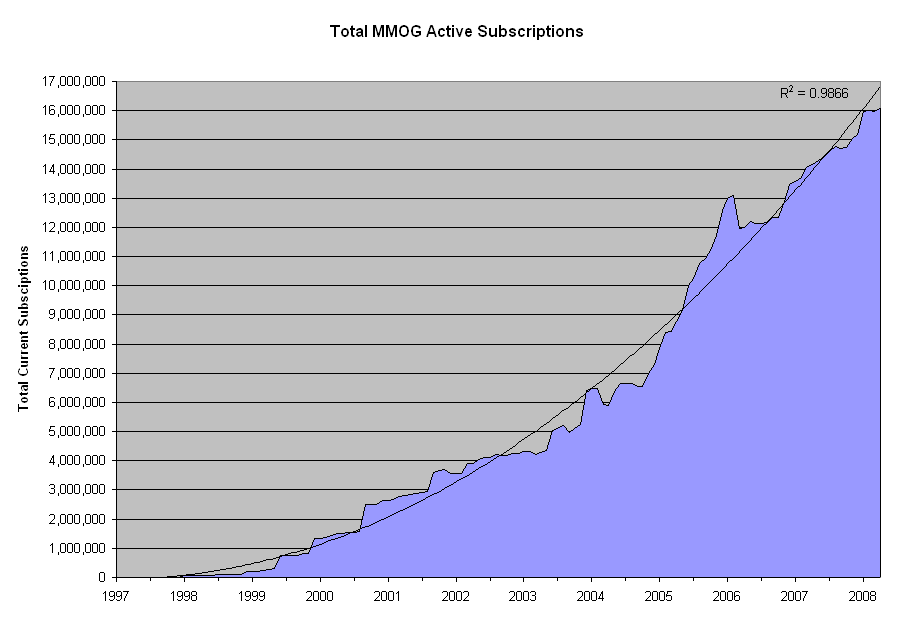
\includegraphics[width=0.7\columnwidth]{MMOG_subscriptions}
 \caption{Total number of active MMOG player subscriptions over time \cite{mmo_growth_chart}.}
 \label{fig_mmog_subscriptions}
\end{figure}

\acp{MMOG} are characterised by expansive worlds, where a large number of players interact online with each other and the virtual environment to achieve certain goals through collaboration and teamwork. Throughout the development of \acp{MMOG}, role play has been tightly coupled to this type of game. This is perhaps due to the exploration and player interaction aspects. Role play allows players to fully immerse themselves in the game world and might, therefore, provide for a more compelling experience. Because of this tight coupling, the terms \ac{MMORPG} and \ac{MMOG} have almost become synonymous. Throughout this work, a distinction will, however, be made between the two.

\acp{MMOG} hold great commercial as well as academic value. From a commercial perspective, the growing number of active subscriptions shown in Figure \ref{fig_mmog_subscriptions} translates to a growing \ac{MMOG} market. Figure \ref{fig_mmog_market} shows the online games market forecast by DFC Intelligence, a company specialising in game market forecasts for various sectors.
%
\begin{figure}[htbp]
 \centering
 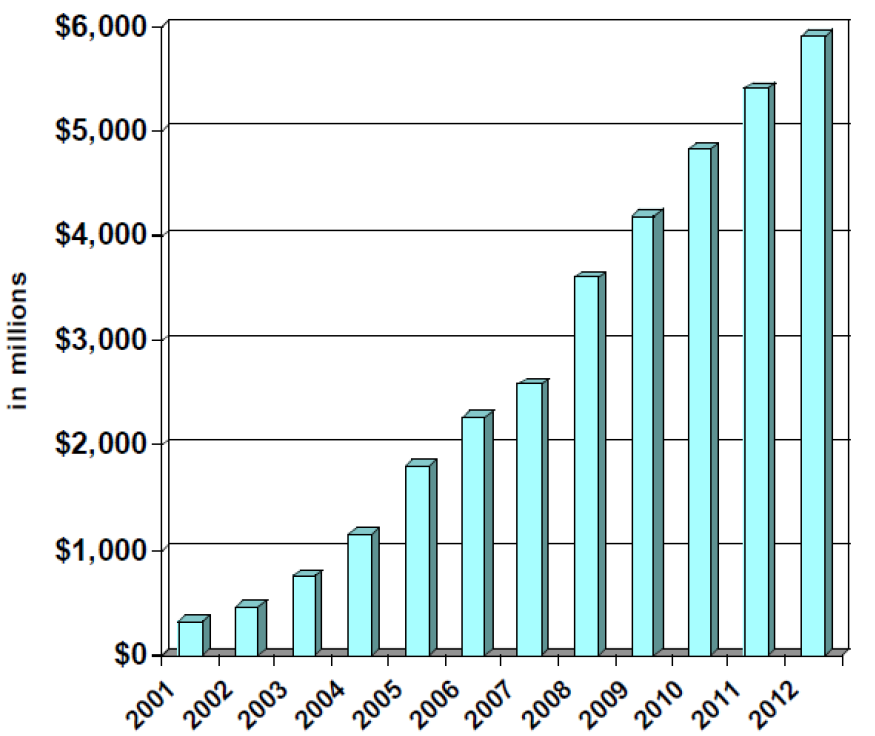
\includegraphics[width=0.4\columnwidth]{DFC_MMOG_market}
 \caption{DFC Intelligence MMOG market forecast '08 \cite{Fan_phd}.}
 \label{fig_mmog_market}
\end{figure}

From an academic perspective, \acp{MMOG} also hold great value. An MMOG is a complex networked application, with clients requiring reliable real-time feedback on actions taken. The design of an MMOG requires in-depth knowledge of server architectures and network design. The design of a server architecture determines how may players the game will be able to host and what the user experience will be in terms of quality of service. The server architecture must be able to handle thousands of requests, store large amounts of data, update the game state and send responses back to all clients in real time.

MMOGs, therefore, hold great academic as well as commercial value. Recently, significant research has been done in order to develop \ac{P2P} MMOGs. These P2P MMOGs hold many advantages over current systems, as discussed in Section \ref{p2p_mmog_overview}. These \ac{P2P} MMOGs, however, still have many issues that need to be resolved before they can become commercially viable, as discussed in Section \ref{key_challenges}.

Part of an MMOG is ensuring low latency, consistent data persistency of all game data. Player data should be stored when players log off from the game. In-game object states should also be stored as well as the states of computer characters in the game. The issue that will be focused on in this study will be ensuring data integrity and persistency in these P2P MMOGs. The question will also be asked which is the better architecture for MMOGs? The classic architecture will be compared to the P2P architecture in order to answer this question. While doing this, a novel architecture will also be developed to improve upon the current P2P architectures by using what was learned from this study.

Section \ref{mmog_history} presents a history of MMOGs in an effort to show the advancement the advancement and major contributors in the field over the past few years.
%
Section \ref{classic_network_models} discusses classic networking models used in current MMOGs. The models are described and the advantages and disadvantages of each are compared.
%
Section \ref{p2p_network_models} introduces the P2P MMOG networking model currently in use. It discusses all aspects of the model and compared different approaches employed.
%
Section \ref{proposed_architecture} proposes a novel P2P MMOG architecture, which makes use of knowledge gained from the development of previous architectures.
%
Section \ref{related_architectures} compares the proposed architectures to related ones and discusses the differences of the architectures and the novelty of the proposed architecture.
%
Section \ref{consistency_models} details how file storage and consistency are handled in a range of systems currently employed.
%
Section \ref{p2p_mmog_cm} details how file storage and consistency are employed in P2P MMOGs. The three different approaches are discussed in detail.
%
Section \ref{proposed_consistency} proposes a novel state persistency model, to support the proposed architecture and improve storage performance in MMOGs.
%
Section \ref{related_cm} compares the proposed consistency model to a currently used model that is most related.
%
Section \ref{evaluation_techniques} describes how the system will be evaluated. Including a discussion of the testing of the architecture and simulation and testing of the consistency model.
%
%Section \ref{expected_outcomes} presents the expected outcomes and contributions of this work.



\section{A brief history of MMORPGs}
\label{mmog_history}

\acp{MMOG} have a history stretching from 1978 to the present. A complete history of \acp{MMOG} and the histories of the games and boardgames that they originate from can be found in \cite{mmog_past_present_future} and Chapter 1 of \cite{designing_virtual_worlds}. The first games that could be called \acp{MMOG} were \acp{MUD} (1978) \cite{mud_intro}. \acp{MUD} are entirely text-based, with players exploring areas by receiving descriptions of what they were ``seeing'' and typing commands to move and interact with objects or players. \acp{MUD} contain many of the elements that today are still central to the \ac{MMOG} concept. These elements include exploration, large worlds, multiplayer, social interaction and progression.

After \acp{MUD}, there were many \acp{MMORPG} that acted as building blocks for what is recognised today as being an \ac{MMORPG}. The first graphical \ac{MMORPG} was Neverwinter Nights (1991) \cite{nwn_aol}. Neverwinter Nights was not an Internet based game, it was hosted on what today is the AOL network. Meridian 59 (1994) was the first \ac{MMOG} to have featured a monthly subscription fee, receive wide media coverage and most importantly, the first \ac{MMOG} to feature a 3D engine \cite{meridian59_hist}.

The first \ac{MMORPG} to be commercially successful and largely credited with popularising the genre was Ultima Online (1997). Ultima Online used existing intellectual property from the Ultima universe as well as an aggressive marketing campaign by game publisher EA, to quickly gain 100,000 subscribers. NCsoft's Lineage (1998) looked similar to Ultima Online, but was more \ac{PvP} oriented and with an added castle siege mechanism, became very popular in South Korea. Lineage had more than three million subscribers at one point, most of them from South Korea \cite{mmog_subscriptions}. Everquest (1999) is credited for bringing \acp{MMORPG} into mainstream Western Culture. It featured a large persistent 3D environment that was capable of hosting up to 15000 players per server \cite{everquest2_capacity}.

\acp{MMORPG} in the first millennium are considered to be of the first generation. These games provided blueprints for all \acp{MMORPG}
to follow in the second generation. While there are many more games in the second generation, these games are characterised by little innovation
in the genre and focus more on improving graphics and ease-of-use \cite{mmog_past_present_future}. Notable games in this generation are: Final Fantasy XI (2000) (console based), Dark Age of Camelot (2001) (realm vs. realm combat) and Anarchy Online (2001) (instancing).

Eve Online (2003), developed by CCP Games in Iceland, brought many new innovations to the \ac{MMORPG}. It was the first successful MMORPG to feature a science fiction theme. It was the first MMOG to have a single distributed server architecture. In 2006, CCP Games launched the largest supercomputer in the gaming industry to upgrade their existing infrastructure and enable Eve to support more than 50,000 concurrent users \cite{eve_launces_supcom}. This number was surpassed in 2009 with 54,181 concurrent users in-game \cite{eve_pcu}.

Another innovation of Eve was the in-game economy. CCP games appointed Dr. Eyj\'{o}lfur Gu\~{o}mundsson as chief economist of Eve online in 2006 \cite{eve_economist}. His duties were to monitor and predict market trends in the game world and produce detailed quarterly economic reports \cite{eve_econ_rep}.  The economy is based on an open market system, ruled by supply and demand. No other game has implemented an in-game economy in such a rigourous fashion.

Blizzards's \ac{WoW} (2004) is the most successful MMORPG to date. After six years it still has by far the most subscribers of any MMOG, totaling 11,5 million, each paying \$15 per month subscription \cite{wow_subscibers}. In 2008 it was estimated that WoW holds more than 60\% of the MMORPG subscription market \cite{mmog_sub_market}. From the first generation of games, a steady growth has been seen in the MMOG space, but before the run away success of WoW, no one had estimated that the gaming market could be this large \cite{mmog_growth_analysis}. It should be noted, however, that the growth seen in the \ac{MMOG} market, is mostly due to growth in the Asian markets and that the size of these markets are much larger than that of Western markets.

The success of \ac{WoW} has largely been attributed to the overall quality and finish of the game \cite{wow_gameplay}. It is interesting to note that WoW is not attributed with many innovations. Most games that came before it implemented most of the features in WoW. What WoW did do, is combine all previous innovations into a package that was accessible to a large number of people.  Players also don't just play WoW to experience the game content, they play the game to meet up with friends and socialise. Guilds are also an integral part of WoW. Guilds are collections of players that choose to play together to achieve some common goal.

All games in the history of \acp{MMOG} can be thought of as a collection of architectures that together make up the game. Architectures can be grouped to form other architectures. The game itself is also an architecture. This proposal will focus on the networking architecture of the game.


\section{Classic MMOG network models}
\label{classic_network_models}

The network architecture, also called the network model of a system, specifies how the different entities in the network communicate, where authority lies and whether a centralised or distributed approach is followed. The networking model used, determines how the different nodes in the network interact and what the roles of these different nodes are. The consistency model used, is based on the networking model, but determines how data are stored on the system as well as how data are moved from one node to another. Throughout this work, data persistency is handled as a subset of data consistency.

Currently, all MMOGs being operated run on a \ac{CS} networking model or a distributed \ac{CS} networking model, also called a \ac{CMS} model. The simplest form of a network model used in MMOGs is the pure \ac{CS} model. Other games, such as strategy games and first person shooter games regularly employ the peer-to-peer networking model to achieve greater system responsiveness, as discussed in Section \ref{classic_models}.

\begin{figure}[htbp]
\centering
 \subfloat[Client/Server]{\label{fig_cs_arch}
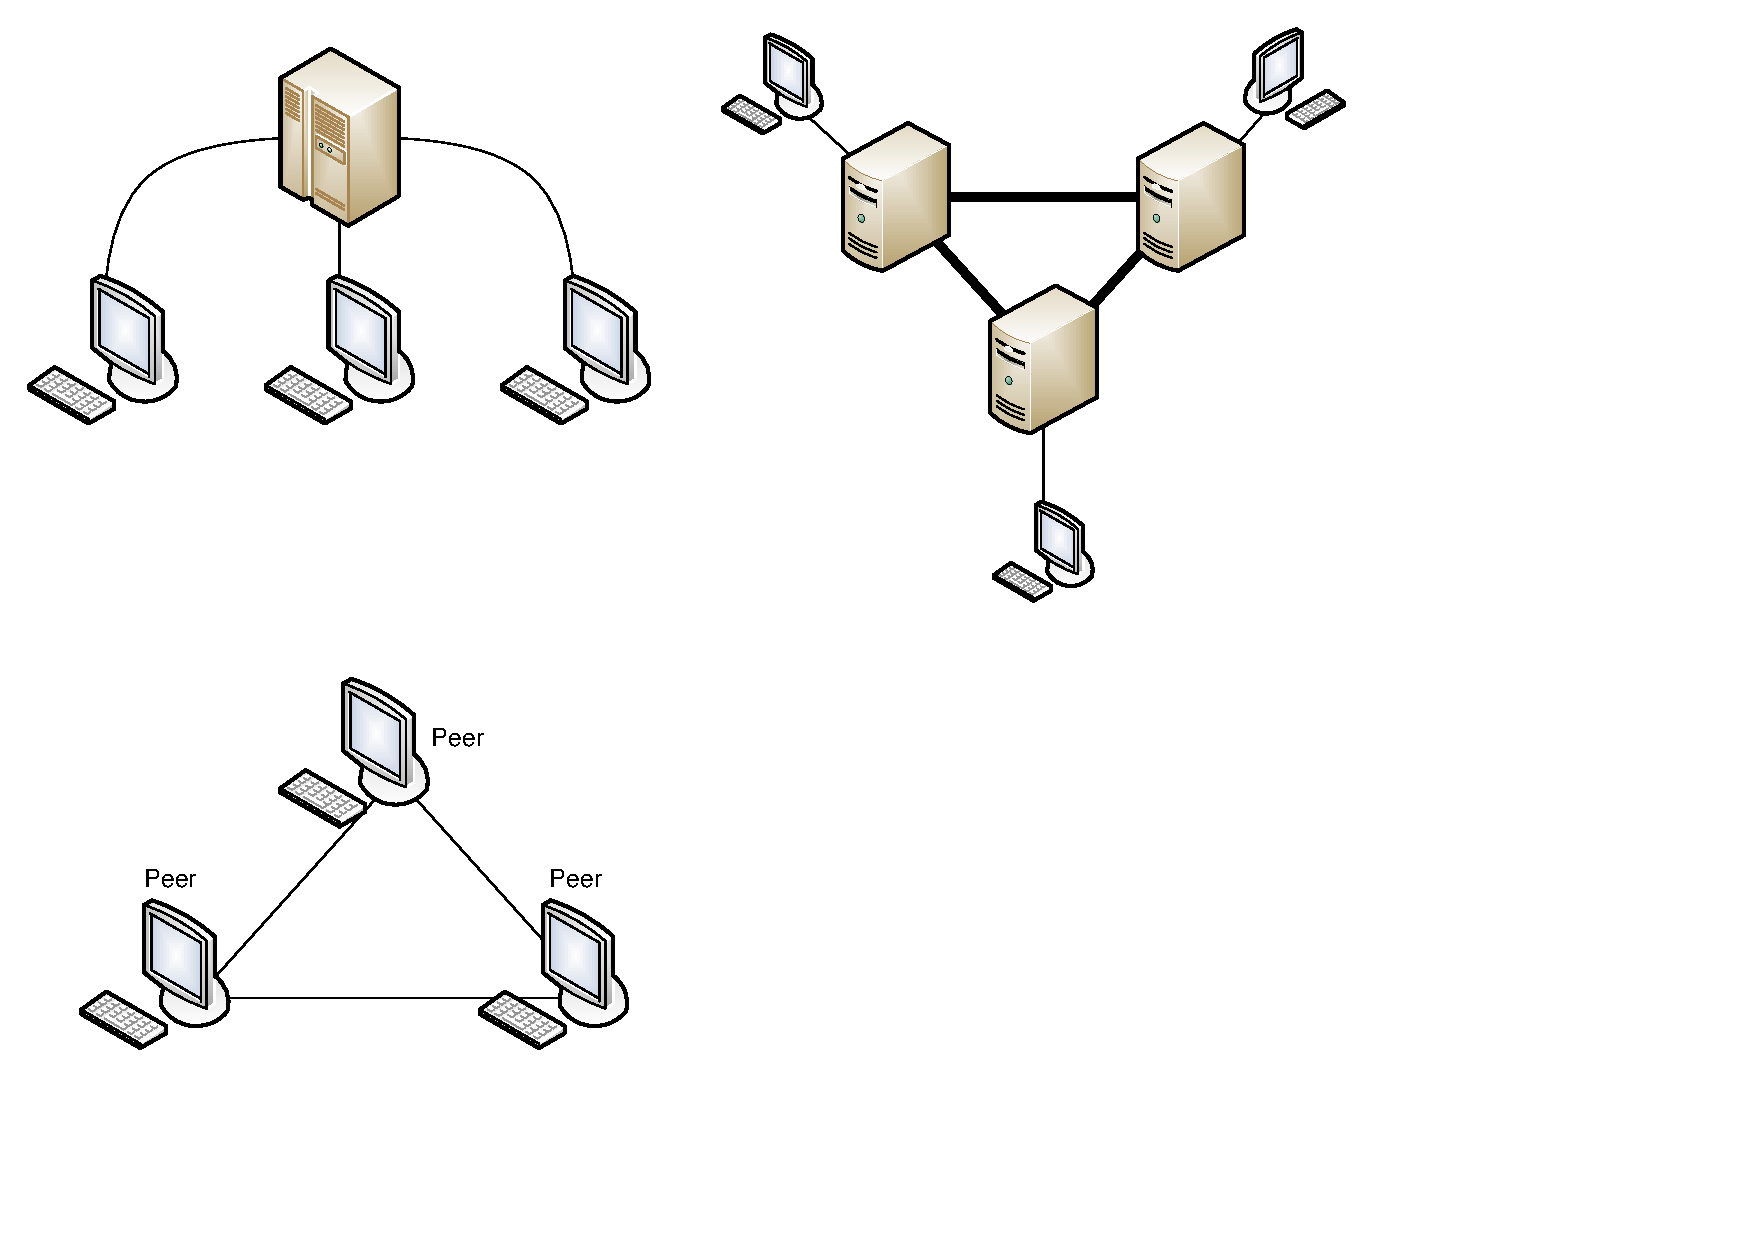
\includegraphics[clip=true, viewport= 0cm 12cm 11.5cm 21.5cm, width=0.5\columnwidth]{network_archs}}
\subfloat[Client/Multi-Server]{\label{fig_cms_arch}
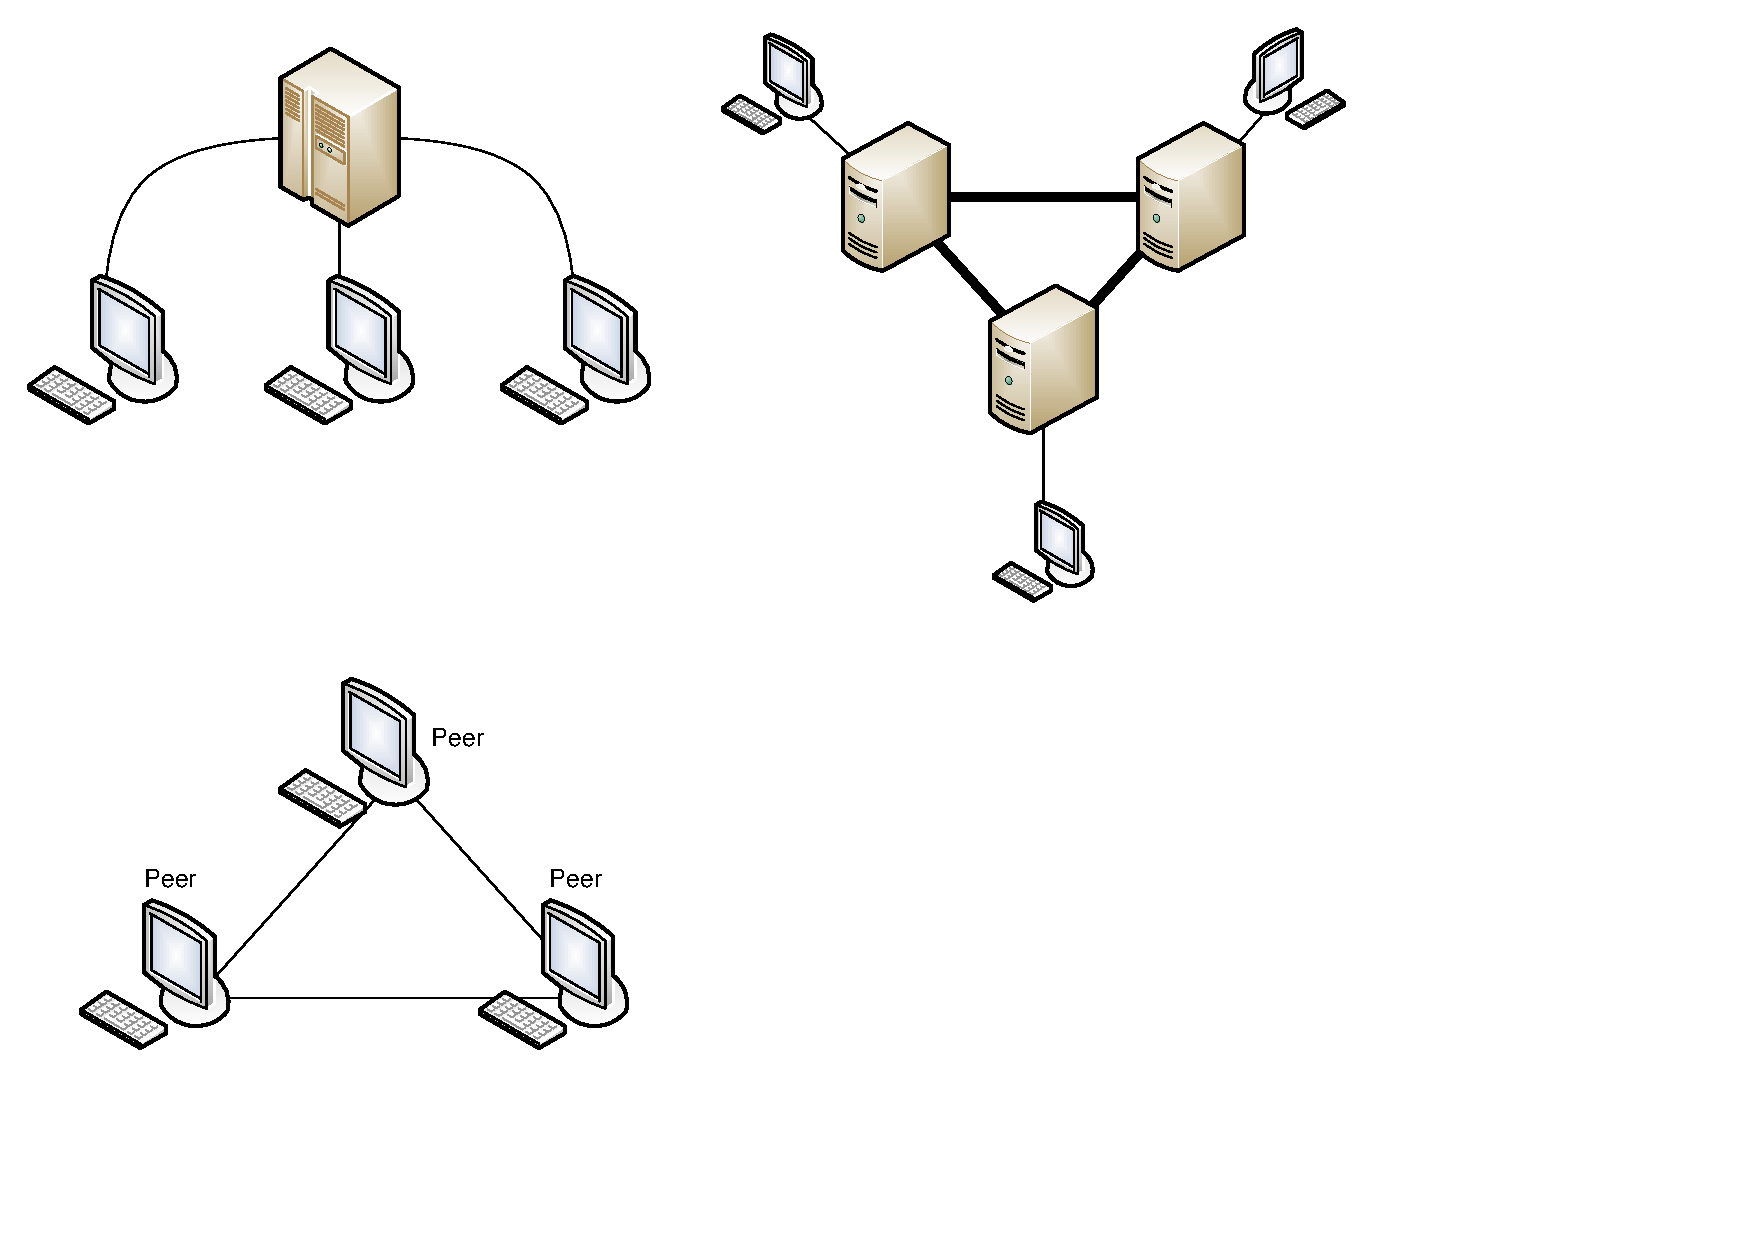
\includegraphics[clip=true, viewport= 12cm 10.5cm 23cm 21cm, width=0.5\columnwidth]{network_archs}}
\caption{Network architectures}
\end{figure}
%
Figure \ref{fig_cs_arch} shows the \ac{CS} model. The server is the entity on which the MMOG is hosted and is controlled by the game producer. Clients are computers operated by players, that connect to the server to play the game. The server is responsible for handling all queries from clients. Clients never communicate with other clients; they send their actions to the server and receive the updated states of other players from the server.

The \ac{CS} architecture has two main advantages that made it the architecture of choice for all MMOG developers. Because of the centralised approach of the architecture, both administration and security are greatly simplified. Administration is simplified, because the game producer has full control over the server, server data and code. Efficient logging is also supported, because the server is able to not only log all server actions, but also all client actions.

Security is a significant issue in MMOGs, since some players sell in-game currency for real-world currency \cite{chinese_gold_farmer}. This makes the MMOG a platform that is capable of producing income, which increases the incentive of players to be able to gain an unfair advantage over others. The more popular an MMOG, the greater the security threat. Because the producer has full control over the server code and is never required to furnish the client with the server code, a potential attacker never has any knowledge of the server architecture and code. Because clients are never allowed to communicate, all malicious users can be filtered out of the network by the server when detected and even banned from the network.

Producers are able to ban players, since these games usually require a game account, which is linked to a copy of the game as well as some payment method. This introduces a large cost to players whose accounts are banned. The server or cluster is also housed in a secured location, where access can be controlled.

These factors simplify the security of the \ac{CS} model by allowing the developers to place all intelligence in the server and move all sensitive computations to the server. This provides the C/S model with a high level of security.

The \ac{CS} architecture however does have some disadvantages. These are: weak robustness, weak scalability, high cost to the provider, high latency, high amount of required server bandwidth and weak handling of transient loads. The robustness of the system is weak because it is a single point of failure. If the server fails or goes down for maintenance, the game is off-line and players are unable to play.

This system is also not scalable, since a single server cannot easily be extended with more resources. Even if an off-line approach is used, where hardware is upgraded after the system is taken down for maintenance, the hardware required to support a game hosting more than 3000 players, become prohibitively expensive. In 2004, it was estimated that an MMOG that supports approximately 30,000 players, requires 2 to 3 years to develop and costs more than \$10 mil \cite{cs_mmog_cost}, \cite{igda_online_whitepaper}. With newer games using high definition graphics and the general drive in the market to improve on previous titles, the cost of MMOG games can only be expected to increase.

The server hardware should be able to support peak system loads, which means that sufficient resources should always be provisioned to support these peak load. This is not an economically viable solution, because resources to handle peak loads are not used most of the time. This translates to producers paying for the provisioning of resources, without having active players that pay for these resources.

This disadvantage also leads to a high cost for the provider, which translates to high costs for clients or reduced profit. The cost is due to the hardware that is required to host the system as well as maintenance and running costs. Running costs include bandwidth provisioning and IT personnel. Maintenance costs include replacement of malfunctioning or outdated hardware. It has been estimated that maintenance and running costs consume approximately 80\% of game revenue during the lifetime of the game \cite{cs_mmog_cost}.

Because no clients are allowed to communicate with other clients, every change that is made to the game world by a client, first had to be communicated to the server, which in turns relays this message to all clients after applying game logic and artificial intelligence (AI) algorithms. This two hop path, with the additional time for computation added by the server as well as possible buffering at the server when many clients communicate, significantly increases the latency of the system compared to a system where direct communication is used.

In an effort to address some of these issues, the distributed \ac{CS}, also called \ac{CMS}, was introduced. In a distributed \ac{CS} model, the server functions are distributed amongst multiple machines in an effort to distribute the server load. The server functions can be distributed by means of redundancy or specialisation. In a redundant system, server functions are duplicated. In a specialisation system, different server functions are handled by different distributed servers.

In general, the issues addressed and improved by the \ac{CMS} architecture are robustness, scalability, and peak load handling. The system is more robust, because the failure of one server will not necessarily lead to the failure of the whole system for certain system designs. The system is more scalable, because many less powerful servers may be used, which allows for the hosting of more players than what is currently possible with single server hardware. It also handles transient loads better, because, for cases where loads can be predicted, resources can by shifter between servers to improve the user experience.

The disadvantages of this system is that the administration complexity is greatly increased. Such systems, although capable of handling many more users than a single server, is also much more expensive. These disadvantages are however not technical problems and so it is assumed for current games, that these systems are what is required if a game is to be hosted for a large number of players.

\section{Peer-to-Peer MMOG network models}
\label{p2p_network_models}

\subsection{Overview}
\label{p2p_mmog_overview}

Recently, an architecture making use of the peer-to-peer networking model to host MMOGs, has gained popularity. This was first formally published in \cite{knutsson_p2p_first}. A new research field has been opened up, which is attempting to make the peer-to-peer model a viable alternative to the classic \ac{CS} and \ac{CMS} architectures. This architecture does, however, still have a few major issues that need to be solved before MMOGs can be developed that use it. If these issues, discussed in Section \ref{key_challenges}, can be solved, a \ac{P2P} architecture holds some powerful advantages over a \ac{CS} system.

The core idea of the \ac{P2P} model is that each peer contributes sufficient resources to the network to be able to host itself. This also means that all functions of the server in the classic \ac{CS} model are distributed amongst all peers. There are many areas where the \ac{P2P} model can improve on the classic \ac{CS} model. These areas are robustness, scalability, provider cost, latency, server bandwidth and handling of peak transient load.

The system is very robust, because there is no server that can fail, only individual peers. Individual peers failing will not affect any other peers other than the peer that failed. This behaviour makes game down-time extremely unlikely.

Also, because every peer is expected to add sufficient resources to the system to host itself, this makes the system very scalable with no extra costs being incurred from a provider viewpoint for any peer that joins the network. This will also allow for efficient handling of transient loads. If many players suddenly enter the game, no resource provisioning issues will arise, as peers already possess their required resources. It should also be noted that it is not at all unreasonable that a peer will have sufficient resources to host itself. Peer computers are very powerful systems these days, with multi-core CPUs, multiple gigahertz of clock speeds, multiple gigabytes of memory and secondary storage space in the terabyte range. The graphics cards in gaming machines have also become immensely powerful.

\ac{P2P} architectures also create a lot of opportunity for independent developers, because a large initial investment is now no longer required to purchase the expensive server hardware. Not just are hardware costs greatly reduced, but running costs are also greatly reduced. The bandwidth required by the game server is now shared amongst users. Which means that no bandwidth costs will be incurred by the provider. Also, the amount of required bandwidth per user is usually not high, which means that users will not be expected to use a much greater amount of bandwidth.

Latency is also improved, because it is now possible to directly communicate between peers and not necessary to go through a server for communications. There is also no single server that has to process peer actions. Peer actions need only be processed by other peers who find the specific peer actions of interest. The distribution of the load as well as direct communication will reduce latency.

There are, however issues with administration and security. From an administrative perspective, it is more complex to administer a decentralised system than a centralised one. For a peer-to-peer system, the server is the collection of all peers. The game producer does not have direct access to peers and so controlling these nodes become significantly more complex. P2P security issues also stem from the decentralised nature of the system and the fact that an attacker has full access to all system code. These issues are discussed in more detail Section \ref{key_challenges}.

Table \ref{tab_archs} summarises the differences between the three architectures as discussed thus far. From this architecture and the precious discussion, it can be seen that the P2P architecture has a lot of advantages over a classic C/S architecture, but that there are issues that have to be deal with.
%
\begin{table}[htbp]
\centering
\begin{tabular}{|r|c|c|c|}
\hline
Property & Client/Server & Client/Multi-Server & Peer-to-Peer\\
\hline
Administration & Simple & Challenging & Complex\\
Security & High & High & Low\\
Robustness & Low & Medium & High\\
Scalability & Low & Medium & High\\
Provider cost & High & Very high & Low\\
Latency & High & High & Low\\
Server bandwidth & High & High & None\\
Peer bandwidth & Low & Low & Medium\\
Peak transient load handling & Bad & Medium & Good\\
\hline
\end{tabular}
\caption{Differences between Client/Server, Client/Multi-Server and Peer-to-Peer architectures}
\label{tab_archs}
\end{table}

\subsection{Structured P2P overlay networks}
\label{overlays}

P2P architectures can be divided into two different types. These are structured and unstructured. The classification is mostly based on routing and content retrieval in the network. Unstructured approaches generally make use of flooding techniques to obtain data items.

In flooding, a query is send out by one node to all of its neighbours. If these neighbours do not posses the item, they send the request to all of their respective neighbours. Various issues have been identified with flooding \cite{overlay_scalable_alternative}. Flooding is unscalable as the number of queries grows exponentially with the number of nodes in the network. Not just is it unscalable, but the node originating the query is not assured that an item residing on the network will be found.

These attributes of flooding make it an unreliable option for use with P2P MMOGs. Structured overlays have been proposed that provide for efficient routing. Some of these well known overlays are: CAN \cite{CAN}, Chord \cite{chord}, Tapestry \cite{tapestry} and Pastry \cite{pastry}. The overlay most used in P2P MMOG systems is Pastry, as Scribe \cite{scribe}, which implements Application Layer Multicast, runs on top of Pastry.

The basic idea of an overlay is that all nodes are identified by unique IDs, which are hashes to a circular key space. Any node in the overlay network is then able to efficiently route a query with a given ID, to a node with an ID closest to the given ID.

Since the introduction of overlays, they have been employed for various tasks. One task is simple message routing, but on top of the routing layer, many other services have been implemented. These include \ac{alm}, distributed storage \cite{past_storage_focus} and indexing. \ac{alm} required the presence of a structured tree to send messages over. Implementations such as Scribe use the Pastry overlay to form a multicast tree over the structured network overlay.

PAST \cite{past_storage_focus} uses Pastry to implement a distributed storage system. Files that have to be stored are given IDs, by using some hash function, for example SH-1. The file, along with the ID is sent as a message over the overlay. The messages is then routed to the node whose ID is a closest match of the file ID, where the file is stored. If any nodes wishes to retrieve the file again, it only required the file hash. It can send a get message to the overlay, which will route the message to where the file is situated and retrieve the file.

Both PAST and Scribe are widely used in P2P MMOGs as will be shown throughout this proposal.

\subsection{Key challenges}
\label{key_challenges}

A recent article has identified six key challenges of P2P systems: Interest Management, Game Event Dissemination, NPC Host Allocation, Game State Persistency, Cheating Mitigation and Incentive Mechanisms \cite{Fan_deisgn_issues_p2p}. Currently, these are the most pressing issues to be addressed in the design of a P2P game. Each of these challenges will be described below, except NPC host allocation. NPC host allocation is handled as a specialised form of state persistency management in this work.

%Some key requirements have also been identified. These requirements stipulate what characteristics an MMOG should poses, to be classified as such. %These are: Distribution, Consistency, Self-Organisation, Persistency, Availability, Interactivity, Scalability, Security, Efficiency, %Maintainability \cite{Schiele_p2p_requirements}.

%Describe key requirements
%Explain P2P overlays

%Describe key challenges
\subsubsection{Interest Management}
\label{key_challenges_im}

Interest management is used to determine the smallest amount of information that a peer requires, in order to present an accurate representation of the world to each player. The idea is not specific to P2P MMOGs and was already formally put forward in \cite{First_IM} and later with greater focus on a distributed environment in \cite{Whang_agent_based_IM}. The main idea is that a player has a limited visual range and a limited area around the player in which it can interact with objects. The player requires update information of all objects in this area, called the player's \ac{aoi}. AoI calculations also rely on the fact the a player's direction and velocity of movement also cannot change instantaneously and are bounded. Extensive research has been done into solving AoI problems and a comparison of techniques can be found in \cite{Boulanger_IM_compare}. The solutions range from aura/nimbus \cite{Benford_spatial_IM} to publish/subscribe \cite{mercury_publish_subscribe} to Voronoi based models \cite{Hu_voronoi_IM}, \cite{Buyukkaya_voronoi_state_management} to hybrid models \cite{hybrid_IM}, \cite{MOPAR}, \cite{fan_mediator_paper}.

Generally, interest management solutions can be divided into coarsely or finely grained solutions, although the hybrid models, especially MOPAR, seem to have gained greater popularity because they seem to have all the benefits of the two solutions and little of the drawbacks \cite{MOPAR}. MOPAR has been shown to perform better than either a finely grained technique or a coarsely grained technique.

Coarsely grained solutions usually divide the game world into multiple regions and when a player enters a region, it subscribes to that region's events. This is called the region-based publish subscribe model \cite{Fan_deisgn_issues_p2p}. All players in the region then receive the region's events, even for players not in their AoI. Finely grained techniques create groups of players from their \acp{aoi}. Groups of interacting players directly exchange information, so all players only receive information that is relevant to them. This has been termed the spatial model \cite{Fan_deisgn_issues_p2p}. The grain of the solution in turn determines the type of event dissemination that should be used, as described later in this section.

MOPAR partitions the game world into hexagonal regions and appoints ``home'' nodes to act as bootstrap nodes for each region. A home node of a region is that node whose ID is the closest match the the region ID. This allows any node to find the home node for a region. A master node is then selected for every region, whose function it is to inform slave nodes of new neighbours. All slaves nodes in a region register at their region's master node. Slave nodes send direction and velocity updates to their masters. Masters communicate directly with other masters if a node is about to enter their region. Masters inform their slaves of a new neighbour. Slaves communicate directly with each other, once identified by a master.

%The issue with the finely grained model is scalability. As nodes join, the number of messages increase quadratically, as previously mentioned. This means that in highly populated regions, too many messages are sent to nodes which can increase latency to unmanageable levels. Highly populated regions will however experience the same issues if no dynamic regioning is implemented.

%Event Dissemination
\subsubsection{Event Dissemination}
Event dissemination deals with how information should be sent to peers after interest management has determined which information should be sent. The first application of event dissemination for online games can be found in \cite{first_GED}. Recently, \ac{alm} and unicast techniques of event dissemination have become popular, depending on the grain of the event dissemination. \ac{alm} is used, instead of router level multicast, because of a lack of general support for this technology at the router level \cite{ip_multicast_deployment_issues}.

ALM is used for coarsely grained interest management techniques, while unicast is used for finely grained techniques. Unicast is not used for coarsely grained techniques, because it is not scalable. For a network with $N$ nodes, $N^2$ messages are exchanges for every player action. ALM, however, significantly increases the message latency in the system, because messages first have to be routed over a P2P overlay network \cite{}. ALM is however preferred over unicast for large numbers of messages, because of the weak scalability.
%Check Badumna

%Cheating Mitigation
\subsubsection{Cheating Mitigation}
\label{key_challenges_cheating}

Cheating mitigation has been identified as a major issue for P2P systems \cite{knutsson_p2p_first}, \cite{challenges_p2p_gaming}, \cite{cheat_proof_event_ordering}. The challenges reside in the fact that peers are not under the control of the game producer. Since all server data are distributed amongst peers, all peers have access to sections of the server data. Peers also have access to the distributed server code. One advantage that can be exploited is that no peer contains all server data and no one peer has more authority than another.

There are various security issues and these are usually divided according to the level of the protocol stack where they occur. The areas that have been identified by \cite{cheat_proof_event_ordering} and expanded upon by \cite{cheating_taxonomy} are: game level, application level, protocol level and infrastructure level. This is consistent with the generally used layered security model \cite{distributed_systems_security}. Game level cheats are ways in which a malicious player may gain an unfair advantage over other players, within the confines of the game. These cheats are usually because of software bugs and some examples are duplication and teleport cheats.

Application level cheats are where malicious players alter the game software to gain an unfair advantage. This is usually done by gaining access to the game state to which they should not have access at the current time. An example of this is map reveal cheats in strategy games. Where the fog of war is removed and the player can observe all the opponent's movements. Other cheats are sometimes used that augment the player's \ac{ui} with extra information that allows the player to make more informed decisions. It is debatable whether these additions are cheats, they are, however, considered almost essential for competitive \ac{WoW} play.

Protocol level cheats are cheats based on the different methods of communicating data across the system. These usually concern dropping, delaying of modifying IP packets to achieve certain outcomes in the game. Infrastructure level cheats concern exploiting the underlying infrastructure on which the games are built. These include hacking the hardware or P2P overlay.

As with all taxonomies, all cheats may not cleanly fit into one if these boxes, some cheats may occur over multiple levels or a cheat with a specific outcome can be implemented differently on different levels. The field of P2P security has recently received more attention than in the past and has started to bear fruit \cite{survey_p2p_game_cheats}. This is, however, an ongoing research field with many issues still open. For an in-depth review of the security issues facing peer-to-peer system in general, refer to \cite{p2p_security_issues}. These issues are the same issues facing P2P MMOGs, with the exception of the game and application layer issues.

\subsubsection{Incentive Mechanisms}

P2P schemes require all players to share resources in order to ensure that the system functions correctly. The issue with this is that players are people who might not want to share their resources, but still benefit from the resources of others. This is where incentive mechanisms become important. The function of these mechanisms is to ensure that all players contribute resources, by incentivised contribution.

All distributed resource sharing models require incentive mechanisms. Torrent systems for example use the tit-for-tat protocol \cite{} to ensure that all people downloading data are also contributing data. Such mechanisms are also required with P2P MMOGs.

\cite{classic_p2p_reputation} \cite{proactive_reputation}

\subsubsection{Game State Persistency}

The issue of game state persistency will be dealt with in detail in Sections \ref{consistency_models}, \ref{proposed_consistency} and \ref{p2p_mmog_cm}. Game state persistency will form the focus of this work. All that might be said at this stage is what was stated by Lu Fan in Section 3.5.3 of a recently completed PhD on the topic of P2P MMOGs: ``Game state persistency if a major challenge for P2P MMOGs as existing P2P storage infrastructures are designed to support file sharing, and seldom fulfil the performance and security requirements of a MMOG. \ldots the persistency area is still immature with many problems waiting for be investigated.'' \cite{Fan_phd}. This is the same person who also identified the issues focussed on in this section.

\section{Proposed P2P MMOG architecture}
\label{proposed_architecture}

We propose to develop a truly distributed P2P MMOG architecture, using hybrid techniques to improve upon current performance. The architecture will be developed to solve the six issues of P2P systems discussed in Section \ref{key_challenges}. Existing solutions to each of the six issues will be combined into a novel architecture, with the exception of state persistency. For state persistency, a completely novel approach will be followed in line with the design of the overall architecture.

At the core of the architecture will be how peers are grouped. The architecture will not use regions to group peers, but rather, make use of the flocking behaviour of players to dynamically group players into flocks or clusters. These clusters can then be used as the nodes in a clustered \ac{DHT}. Hybrid mechanisms can then be used to either interact with players at the individual level or the cluster level. Because of the flocking behaviour of players \cite{flocking}, dynamic groups or regions that move with groups of players may be a better fit than static or even dynamic regions that operate on areas of the virtual world and not on how groups of players actually cluster.

For Interest Management, a hybrid approach will be followed such as MOPAR. A hybrid interest management technique will fit well with the proposed architecture. The only difference is: where regions were previously used, groups will now be used. MOPAR's direct communication communication between peers reduces bandwidth usage in the network, because at this level, a finely grained interest management technique is used. The structured overlay does however assist in ensuring that all peers remain connected or able to reconnect if they have become disconnected by use of the home node.

We believe that a scheme where the regions or groups move with the groups of players will enhance the functionality of the interest management scheme. If players are grouped more intelligently, less traffic will have to flow between groups, which will reduce the number of queries to the DHT, which in turn will improve the latency of the overall system. Using groups or flocks would, therefore, compliment this technique. The issue with such a system would be how to uniquely identify a group and how the identification would be applied when groups merge or split. The identification is required in order to ensure that disconnected nodes are able to reconnect, once they have joined a group.

As Game Event Dissemination is closely coupled to the Interest Management technique, unicast will be employed. Unicast is used between all master nodes as well as between all slave nodes in MOPAR. Unicast holds many advantages over ALM, if the number of neighbouring nodes are bound. ALM introduces significant delays into the communications system, by the use of an overlay such as Pastry requires $O(\log_{2^b}(N))$ maximum hops to route a message to a target. Where $b$ is usually chosen as 4. While this is sufficient and indeed a good order complexity for routing, in a latency critical application such as an MMOG, this is not sufficient. Unicast, in contrast, provides an $O(1)$ routing complexity. And the fact that groups are used, allows for the unicast group size to be bound.

Security is also of great importance to the design of an MMOG architecture and so security issues will be kept in mind when designing the MMOG architecture. Recent advances and surveys can be used to improve game security, by improving the security of currently used peer-to-peer overlays. Examples include using secure node ID assignments, by making use of a Certification Authority, or designing the system in such a way that a peer cannot select or report it's own node ID. All aspects of security will be investigated, this includes Authentication, Authorisation, Data Integrity, Confidentiality, Availability, Trust, Privacy and Identity Management \cite{distributed_systems_security}.
%Current schemes usually only handle one or two of these requirements as will be discussed in Section \ref{current_architectures}.

%Proposed Incentive mechanisms
Incentive Mechanisms are also of key importance in a P2P system. If peers are not required to share resources, this will lead to system degradation. Two factors should however be addressed: How will resource provisioning be incentivised and more importantly, how will this scheme be made secure. In other words, the scheme should not only ensure that resource provisioning is incentivised, it should also ensure that peers are not able to cheat the incentive mechanism, by providing false information to other peers.

The focus of this work will, however, be on game state persistency. This is an area that has not received much attention in the P2P gaming field. Significant focus has been placed on Interest Management, Event Dissemination and, to a lesser degree, on Cheating Mitigation. The proposed state persistency mechanism is discussed in detail in Section \ref{proposed_consistency}. As an overview, a distinction will be made between ephemeral data and persistent data. A peer-to-peer overlay will be used to securely store persistent data, while a distance based approach will be used to store ephemeral data in a group or flock of peers. This will allow for high speed game state updates for peers within the same group, but the structured approach will still ensure the availability of the game state to other flocks of players, to a lesser state of consistency. It is also argued that players not near to each other, do not require a perfectly consistent view of the complete world. As different flocks near each-other, the degree of state consistency will become higher until the groups merge and the sates are consistent.

It is argued that NPC hosting is a specialised form of state persistency. NPCs are seen as objects with logic and state, both of which are data that has to be stored. This merely requires for the definition of game state to be expanded, as elaborated upon in Section \ref{classic_models}. Object logic is both something that has to be stored as well as executed. The question of how and where object logic should be executed should also be investigated.

\section{Related P2P MMOG architectures}
\label{related_architectures}

As the field is still very young, few, if any, complete P2P MMOG architectures have been produced. Some papers describe their work as being a full architecture, but then goes on to only describe one aspect of the implementation. In those circumstances, source code is also not available to help determine whether a fully working architecture has been implemented.

Many of the papers reviewed only describe a partial implementation a P2P MMOG, even if presenting the solution as a complete one. Some articles describe sate persistency, as discussed in Section \ref{p2p_mmog_cm_overview}, others describe interest management as presented in Section \ref{key_challenges_im}, still other describe security issues as presented in Section \ref{key_challenges_cheating}.

Few implementations could be found that attempt to implement a complete P2P MMOG implementation. These implementations are Mediator (2007) \cite{Fan_phd}, VAST (2007) \cite{VON_VAST} and Badumna (2009) \cite{badumna_engine}.

VAST uses Voronoi-based interest management techniques with unicast event dissemination. Unicast is usable in this case because of the small neighbour sets present in the Voronoi-based approach. It uses a distance-based NPC hosting mechanism, but centralised state persistency.

The Mediator framework employs MOPAR-like hybrid interest management with unicast event dissemination. It implements a task sharing approach to NPC hosting, where NPCs are represented as tasks that require computing power. These tasks are then advertised by a specialised super peer. Tasks can be undertaken by peers with sufficient computing power. It implements state persistency by using PAST overlay storage.

The recently developed Badumna uses a three tiered interest management technique. The three tiers are called: ``Cell'', ``Dynamic Bounded Region'' and ``Gossip''. These are techniques based on the aura/nimbus design. Different techniques are used for different network conditions. As player density increases, interest management moves from cell, to dynamic bounded region, to gossip.

In the cell protocol, where all peers start out, the virtual world is divided into regions, with region manager super peers. These super peers maintain lists of nodes in their regions and provide these lists to nodes entering the region. When too many auras intersect, dynamically bounded regions are formed. This is done by grouping peers in some way that is not explained and adding these groups into the regional cells. Another tier is effectively created, with each group having a super peer and a group also being an entity in the virtual world. A group with an area of interest (AoI) is then inserted into a region and when the AoIs of groups overlap, the super peers in the groups are informed. These group super peers then inform the other peers in the group. This approach is used in an effort to decrease network traffic. The gossip protocol attempts to avoid overloading the regional super peer by reducing the rate at which peers query the super peers and allowing normal peer nodes to broadcast their information to their neighbours. It is not clear how this tiered scheme performs to other schemes as this is never compared. Only the different tiers are compared.

In \cite{badumna_engine}, where Badumna is described, it sometimes seems that Interest Management, Event Dissemination and State Consistency are confused for the same thing. Interest management techniques are described as being multicast-based or DHT-based. Apart from the fact that multicast-based schemes usually are also DHT-based, the paper seems to describe DHT-based schemes as state persistency schemes, rather than interest management schemes. Where the example objects (cat, dog, and cat and dog) are stored somewhere on the network. No mention is made here of actual interest management, which is how to determine what is of interest to which peers in the network.

It is also said that multicast schemes are not suitable for interest management, because of the high transmission latency, which is true. But the paper than goes on to state that DHTs are very suitable for interest management, because of the lookup features. No mention is made here that DHTs posses the same latency as multicast, mostly due to that fact the high multicast latency stems from the use of DHTs.

What Badumna does provide, is a usable implementation of a P2P MMOG network suite that is currently being implemented for commercial use in Vastpark, is integrated with the Unity game development tool and OpenSim, and has been used to create a working technology showcase, called ``Troll Basher'' \cite{badumna_showcase}. Badumna does not seem to be a complete implementation of a P2P MMOG architecture, but it allows developers to use it as a base to develop a complete P2P MMOG architecture on.

Issues of state persistency seem to be left up to the developers. It provides functions to create game objects and to ensure that these objects are synchronised with other duplicate and non-authoritive objects. Where the authoritive objects are stored, is left up to the developer. This system could thus provide the base to implement a P2P MMOG architecture on, using novel state persistency and consistency mechanisms. Which is exactly the novel contribution of the proposed work.

None of the architectures reviewed have investigated dynamically grouping peers in a natural way, in an attempt to use the flocking behaviour of peers.

%Remember to talk about security in P2P overlays


\section{Classic consistency models}
\label{consistency_models}

A consistency model is based on the network architecture, but deal with how data is stored and distributed throughout the system. The consistency model specifies on what type of nodes what types of data are stored and also how data consistency is ensured with multiple node requests.

To understand consistency models, some basic terms should first be understood. These terms are: ``event'', ``update'', ``game state'', ``game logic'' and ``game object''. Events are generated by players and can be thought of as actions taken by players. These include casting a spell, using an item or walking. Game logic is applied to events to determine what updates should be applied to the game state. Game logic is thus a think function, which determines how the world should change as a result of an event. Another way to think about game logic is to see it as the game rules. A player casting a spell might cause another player's health to be reduced, her own health to be increased or a monster to spawn. When a player is walking, the logic will cause the player's position to update at the speed, which the player is able to walk.

Game logic communicates how the world should change via game updates. Game updates are the deltas that specify how the current state should change. By now the concept of game state should also become clear. The state of the game is the positions, health and all other attributes of all players and NPCs in the game world. Game state consists of a collection of game objects. An NPC as well as a immutable plant are both examples of game objects that together make up the game state. When discussing how to segment game state, it is sometimes easier to speak in terms of game objects, since they are more finely grained.

For the purposes of this work, game objects are objects with both state and logic, which means they consume both storage space, as well as CPU power. Game objects can also produce events, which should be sent to other objects. When this definition is used, NPC objects may be classified as a specific type of a game object, which forms part of the global game state. The question of NPC hosting then also becomes a question of state persistency.

\subsection{P2P and C/S consistency models}
\label{classic_models}

As an introduction to consistency models, an overview of the two common models, currently used in computer games will be described. The models used in P2P MMOGs are all permutations of these two basic models. The two models are based on the two different network models. These are the P2P-based model, also called the event-based model \cite{p2p_cm_aoe}, and the Client/Server-based model, also called update-based model \cite{unreal_networking}.

\begin{figure}[htbp]
\centering
\subfloat[Peer-to-Peer (update based)]{\label{fig_p2p_cm}
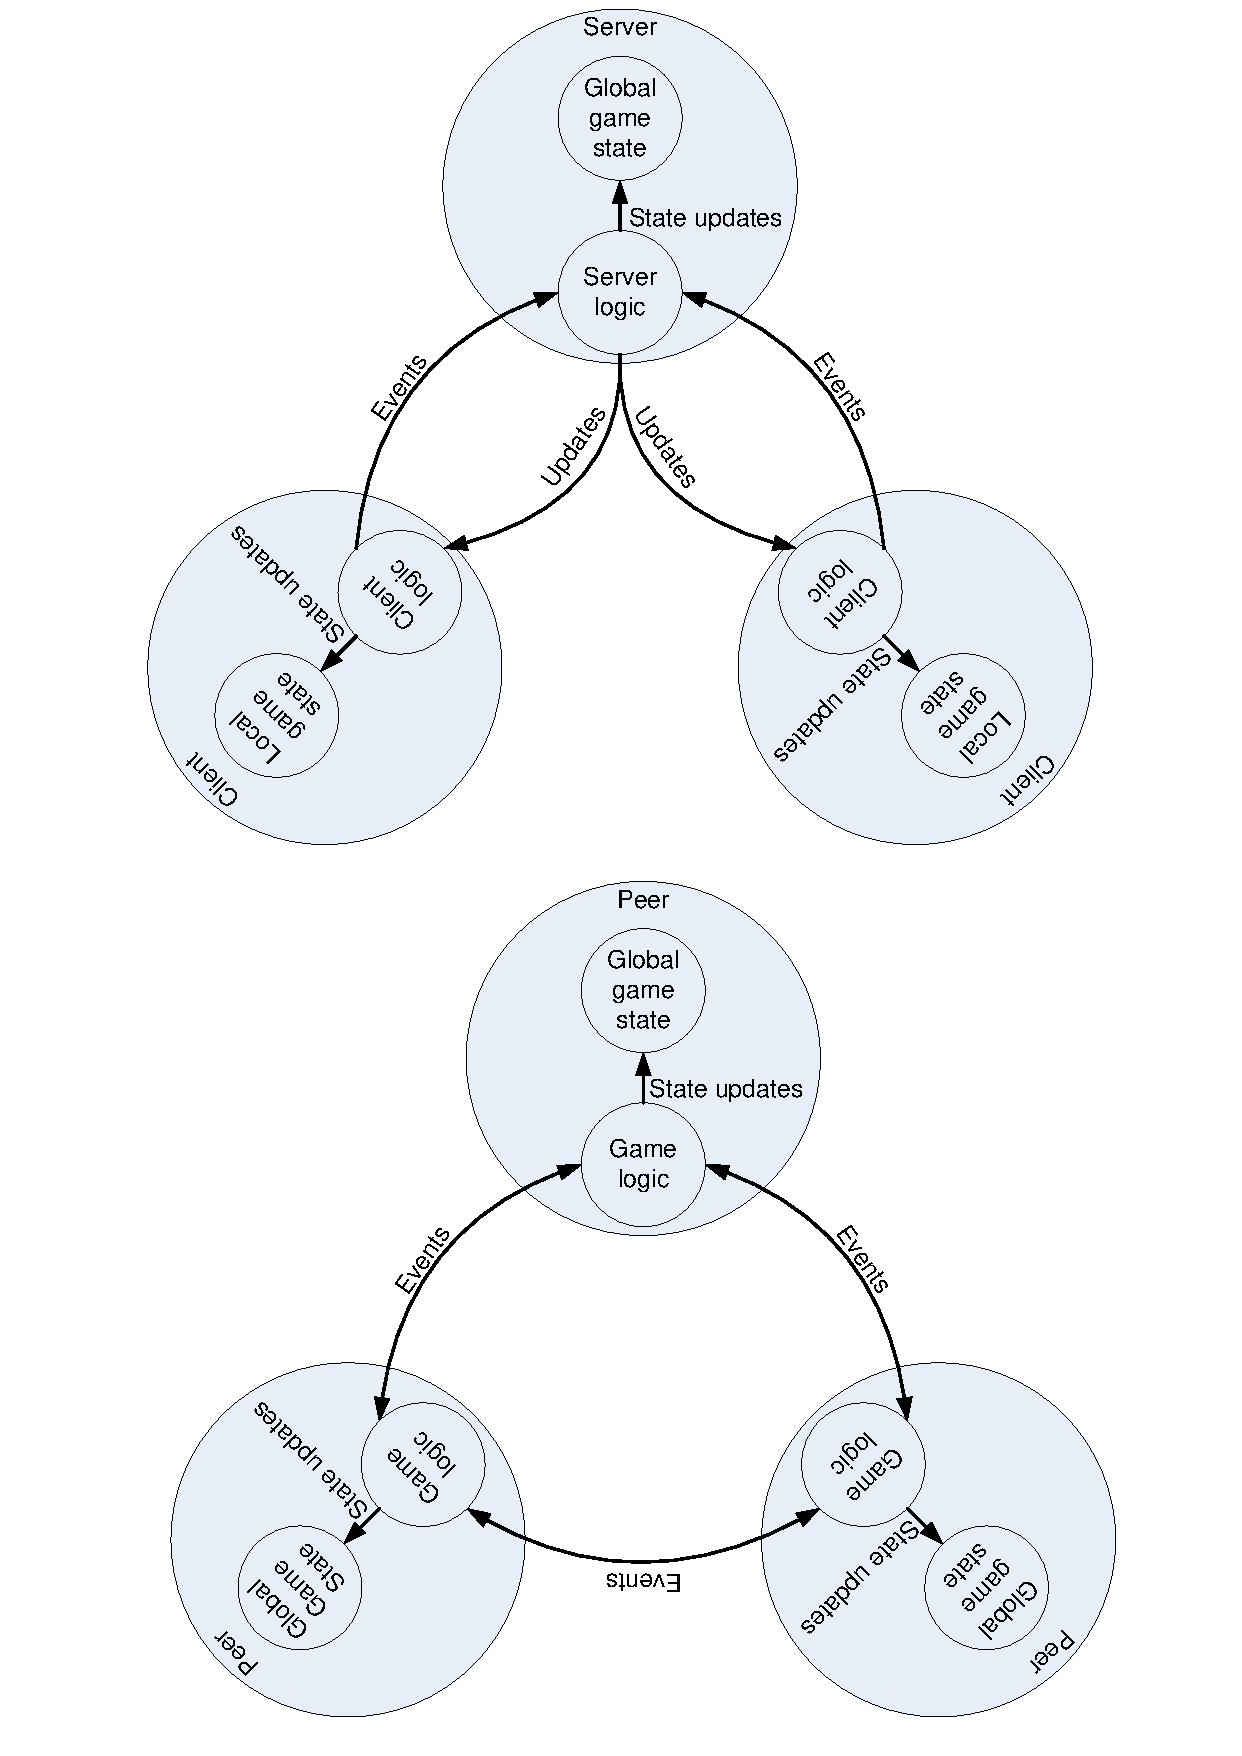
\includegraphics[clip=true, viewport= 2.5cm 0.5cm 19cm 15cm, width=0.5\columnwidth]{CS_P2P_CMs}}
 \subfloat[Client/Server (event based)]{\label{fig_cs_cm}
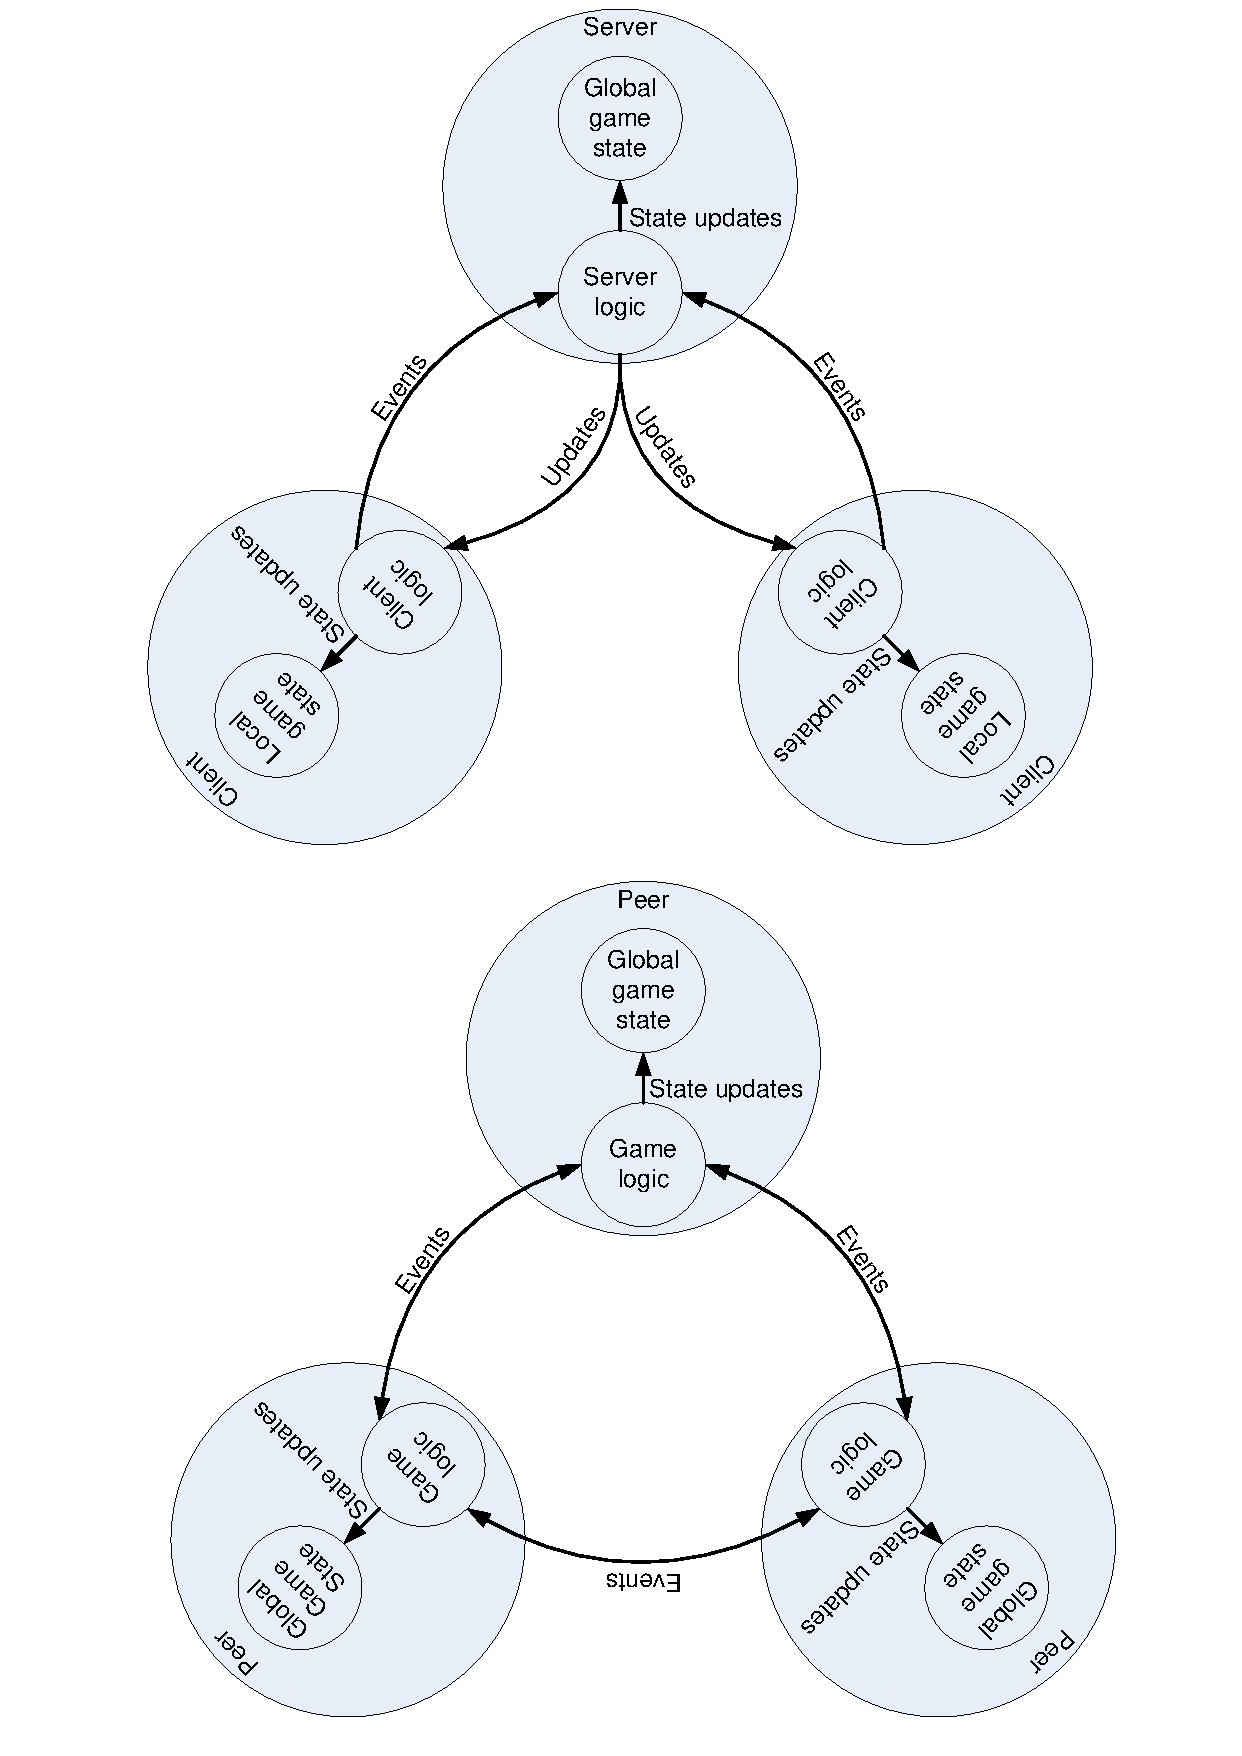
\includegraphics[clip=true, viewport= 2.5cm 15cm 19cm 30cm, width=0.5\columnwidth]{CS_P2P_CMs}}
\caption{Consistency models}
\end{figure}
%
Figure \ref{fig_p2p_cm} shows the P2P model. In this model the complete game state is stored on each peer \cite{}. Any event that a peer generates is sent to all other peers. These events are used as inputs to the game logic, which creates updates, which is used to update the global game state at each peer.

It is at this level that consistency becomes important. The order in which updates are received should be the same for all peers, otherwise the game states of different peers may become inconsistent. Usually some kind of lockstep technique is used to solve this issue \cite{pessimistic_lock_step}. The issue with lockstep is that it reduces the latency to twice that of the peer with the highest latency. Various techniques have been proposed that improves the latency by introducing some deadline before which all events should be submitted \cite{cheat_proof_event_ordering}. This, however, makes it impossible for a player with a high latency to play the game with anyone other than from her own continent.

The issue with the event-based model is that it is not scalable, since all peers should connect to all other peers and every event is transmitted everyone. This means that as $n$, the number of peers in the network, increases, the amount of traffic increases with a factor of $n^2$. The security issues of the P2P networking model, on which this consistency model is based, are also present. Slowdown is also experienced by all players if one player's latency is below par, since the lockstep mechanism has to wait for all events to be received for that round to conclude.

An alternative to the event-based model is the update-based model, shown in Figure \ref{fig_cs_cm}. This model is based on the Client/Server networking model. An authoritative global game state is housed on the server and a non-authoritative local game state is housed on all clients for display purposes. No real game logic is housed at the clients, only on the server. All clients send events to the server, which applies the game logic and sends updates to the clients, while also updating its own game state.

This approach greatly assists with security, as clients cannot influence the state of any other clients and every client's state depends on updates received from the server. The server state is also termed authoritative, because if there is a conflict, the server state is always the state to which the system is expected to return. All the security advantages of the \ac{CS} model also apply to this consistency model. Another reason why the event based model is successful is because it is more scalable then the pure P2P model. More hardware can be used to build a more powerful server, which can handle more client.

\subsection{Client/Multi-Server consistency models}
\label{cms_models}

%Should I add diagrams here?

Apart from the two classic models, there are also models based on the \ac{CMS} network model. There four are are shard-based, replication-based, object-based and zone-based \cite{Hu_voronoi_IM}.

Sony introduced the first consistency method for a \ac{CMS} network in Everquest, where copies of the game world ran on different servers and players connected to one of these servers \cite{engineering_everquest}. Sony termed this method: ``Sharding''.

Clients are not able to interact or communicate with players on other shards, which reduces game immersion. This method does, however, allow for a more scalable system as maximum load is fixed. Players are not able to enter a shard if that shard has reached it capacity. This has in the past caused unhappiness amongst players, since popular shards could be difficult to log in to. Players are also reluctant to move to a new shard, because a lot of time is invested in their characters in their ``home'' shard. Sharding, however, wastes more resources, as one shard may be overpopulated while another is underpopulated. There is no way to dynamically distribute the available resources from one shard to another. For all practical purposes, this approach is still merely a \ac{CS} approach, with players forced into a specific \ac{CS} environment.

%Redundant
The second model is very similar to sharding, with the difference that all servers share the same duplicated game state. Each server contains the global game state and clients connect to any one of these servers (mirror-servers \cite{mirrored_server}) or through a load distribution algorithm to a server (proxy-servers \cite{proxy_server_dist}). Each server handles all actions from clients and updates its own database. The servers in turn send updates to each other over a high quality link, such as fibre, to maintain database consistency at high speeds. The problem with this system is that the world is never truly consistent and that there are no optimally chosen inconsistency obfuscation boundaries. In other words, two players standing next to each other in the virtual world, might be on different servers and, therefore, experience two different worlds. Game inconsistency is not necessarily an issue, but then it should be based on a distance based approach where the consistency degrades gracefully the greater the distance between players in the virtual world. This system is also not truly scalable because of the large hardware costs involved in the system as well as network hardware required to achieve sufficient performance for large numbers of players.

%Object based
The object-based method distributes all in-game objects amongst the servers \cite{object_based_consistency1}, \cite{object_based_consistency2}, \cite{object_based_consistency3}. For an MMOG, most of these objects are expected to be players objects. The advantage of this method is that the system load is fixed for a certain player population and that the load is equally distributed amongst all server. This allows for more accurate prediction and provisioning  of required resources, but still does not handle transient loads well. Another issue is inter-server communications for this architecture. The inter-server communications are random and also much more than the inter-server communications for a region based system. The reason for this is that the amount of player interaction increases with a decrease in the distance between the players. Players playing together move together, chat and interact with \acp{NPC} together. For a region based model, all player-neighbour interaction remain in the server.

%Zone-based
The zone-based method divides the virtual world into zones or regions, which are hosted on different servers \cite{zone_based_stat}, \cite{zone_based_dyn}. Busy regions are hosted on their own servers, while multiple quiet regions are hosted on a single server. This is termed the static region approach \cite{zone_based_stat}. The issue of this static region approach is that it does not scale well when one region is suddenly populated with players. This type of behaviour happens quite regularly and is known as flocking \cite{flocking}. When players find something of interest in a region, many players will flock to that region. In-game events and festivals are also becoming popular and these events also cause flocking to the region where the event is held. The solution to these effects have been over provisioning of resources to handle peak loads, which suffers from the disadvantages discussed above. Also, if the load changes, the server has to be brought off-line in order to balance the regions. Dynamic regions are being investigated, where regions can be dynamically shifted from one server to another, in order to balance load \cite{zone_based_dyn}. This approach adds overhead and significant complexity with regards to the migration of the data and the handling of player actions while the data are in transit.

As will be seen, P2P MMOG models are merely permutations of the classic and \ac{CMS} consistency models.

\section{P2P MMOG consistency models}
\label{p2p_mmog_cm}

\subsection{Key Challenges}
\label{key_challenges_cm}

%Consistency issues
The key challenges related to P2P MMOG consistency models identified during this literature study were: reliability, responsiveness, security, fairness and consistency.

For the storage to be reliable, it must not be possible for data to be lost, and stored data should always be available when a node requests it.

To ensure system responsiveness, data must be stored or retrieved in real-time. With real-time, it is meant that data should be available within a certain time frame that would ensure correct functionality of the MMOG requiring it. The variance in times when data become available should also be small.

The storing system should store data securely. It should not be possible for data to be altered in ways that are inconsistent with the game rules. It should also be possible to identify nodes that alter the data in this malicious way. This also adds the requirement that nodes should be authenticated in the storage system and that only authorised nodes should be able to alter data.

Ensuring fairness in the system means distributing load evenly according to the abilities of individual nodes. This ensures that not only a small number of nodes provide all system resources required for the system to function, but that all nodes contribute what they can, in order to support the system.

The consistency requirement specifies that nodes should perceive the game world as the same. This is intentionally a vague requirement, as it is believed that the stricter requirement of the game world actually being the same is too strong. When two players are playing together, they should perceive the world exactly the same way. If, for example, one player perceives a monster and starts to attack it, while the other player sees nothing, the game experience of both will degrade. As another example, if there is a damsel in distress in a tower for a player that visits the tower, but no damsel for a player that does not enter the tower, the game experience would not degrade. This is because the player not in the tower does not have to know about the damsel. From these two examples, the reason for state persistency based on perception, rather than reality shown.

All state persistency models will be reviewed with these issues in mind.

\subsection{Overview of approaches}
\label{p2p_mmog_cm_overview}

%Overview of three approaches
Very little work has been done on state persistency for P2P MMOGs. Generally three approaches have been identified for state persistency: super peer storage \cite{knutsson_p2p_first}, overlay storage \cite{Douglas05enablingmassively}, \cite{using_freenet_storage}, \cite{overlay_storage1}, \cite{Fan_phd}, \cite{past_storage_focus} and distance-based storage \cite{Buyukkaya_voronoi_state_management}, \cite{Hu_voronoi_IM}, \cite{colyseus_distance_based}. Hybrid techniques, distinguishing permanent data from ephemeral data have also been proposed \cite{zoned_federation}.

\subsection{Super peer storage}

%Super peer storage - description
Super peer storage relies on the super peer storing all relevant information in its domain. An example of this is in \cite{knutsson_p2p_first}, where the world is segmented into regions and super peers act as regional servers to all peers in their region. Each super peer handles all game logic and distributes updates to all peers in its region. The super peer also handles state persistency for its region, hosting NPCs, objects and persistent player data.

\begin{figure}[htbp]
 \centering
 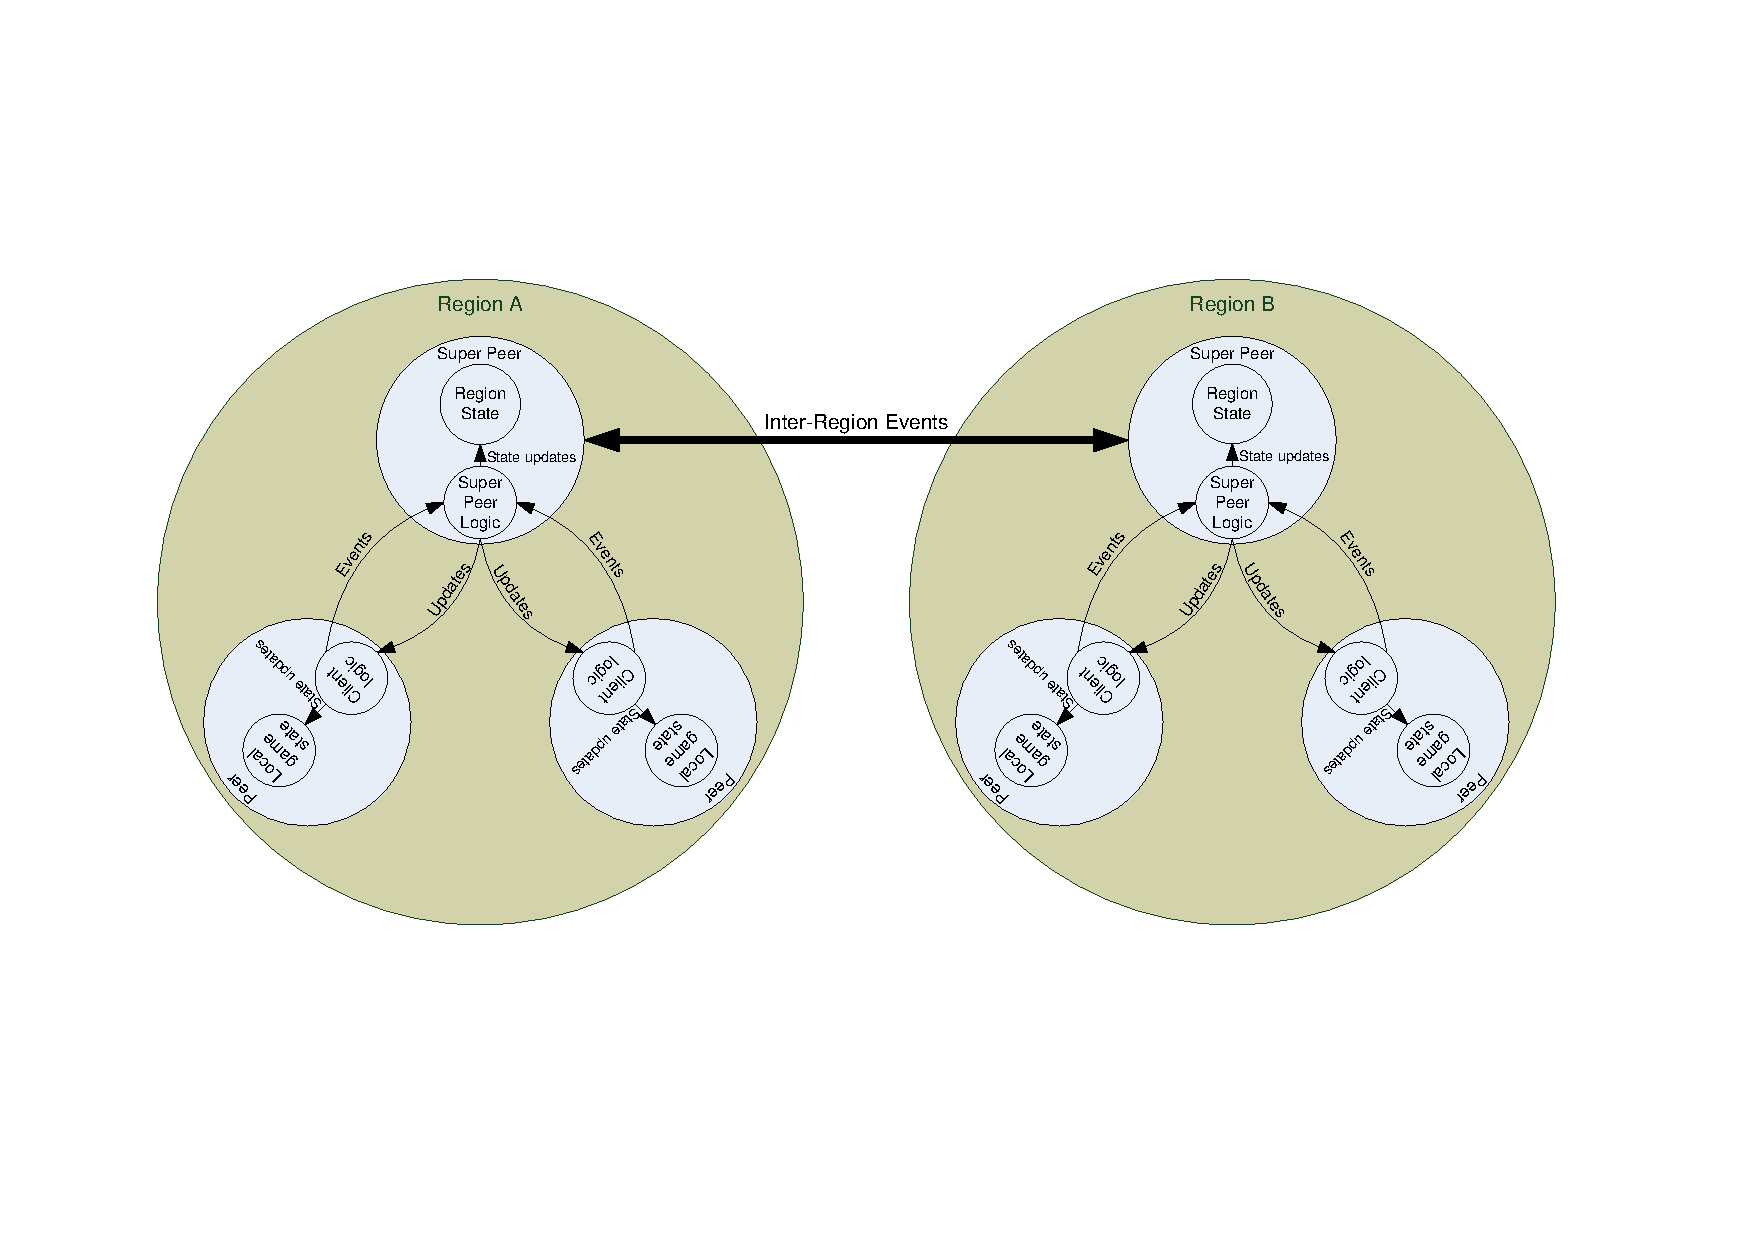
\includegraphics[clip=true, viewport=2cm 5cm 27cm 16.5cm, width=\columnwidth]{region_based_CS_CM}
 \caption{Region-based Client/Server consistency model}
 \label{fig_cs_region_cm}
\end{figure}
%
The consistency model for this approach is depicted in Figure \ref{fig_cs_region_cm}. One can see that this approach is modelled on the update based model, but segmented into separate regions. The role of the server is here fulfilled by a super peer, which is a peer that is selected in some logical way, from the available set of peers and then promoted. Server selection in itself is a complex topic that has to deal with determining whether a peer has sufficient resources available and also whether the peer is trustworthy.

Each super peer in this model houses the complete region state as shown. Super peers also house the real game logic. Clients in the region only house copies of the regional objects and some client logic to update the local copies of objects housed. Like the \ac{CS} model, clients only send events to super peers, where super peers apply the game logic and send state updates to clients.

%Super peer storage - issues
The super peer storage model has many potential issues. Overloading of the super peer is one. A super peer could be relatively easily overloaded if a region becomes too crowded, since a super peer is merely the computer of some player in the game and not a specialised server machine. The question of fairness also arises. The idea of a P2P MMOG model is that all peers share resources. With this model, peers with extra resources are expected to donate these resources for the good of all. Players might consider it unfair, when they are constantly expected to donate resources, some of which they might have to pay for.

Another issue is reliability. In a P2P system, with a high rate of churn, players are expected to constantly leave and join the network. Because of this reality, redundancy mechanisms have to be developed that would ensure state data are always available, even when a super node leaves the network. It is possible to solve these issues by having redundant super peers in each region, that take over hosting responsibility if the main super peer leaves. This has been mentioned in the literature, but no concrete schemes of data migration have been presented \cite{}. Other schemes to support improved reliability deal with reputation mechanisms for super peers. Super peers that have more resources and stay in the network longer are preferred during super peer selection, using reputation mechanisms \cite{fan_mediator_paper}.

The third, and probably most important issue is that of security. If a single peer is allowed to house the player information of a large group of players, it might become possible for such a peer to modify the data to suit his own ends. The issue is not only that modification of the data might be possible, but also that it would not be possible for the cheating to be detected, because of no centralised logging. A scheme that would improve the reliability of this systems has been proposed, where every event is also sent to the backup super peer of the region \cite{past_storage_focus}. The main super peer responds with the update and the backup super peer responds with a hash of the update. A peer can then check whether the hashes match to determine whether the data has been received correctly. A hash is not the state update itself, so will be much smaller, but the events that have to be sent to all super peers will significantly increase traffic in the network and bandwidth usage by peers.

There are, however, also advantages to super peer storage. All data are stored on the super peer, which means that storing data is a low latency operation. The regional state can be stored and retrieved at very high speeds, making the system very responsive. Data retrieval from such a storage is also relatively fast. As fast as data retrieval from a server. Peers can request data from a super peer and the data can be returned to the peer in one hop after transmission of the request. Super peers may, however, become overloaded with requests and thereby increase the latency of the system.

\subsection{Overlay storage}

%Overlay storage - description
\begin{figure}[htbp]
 \centering
 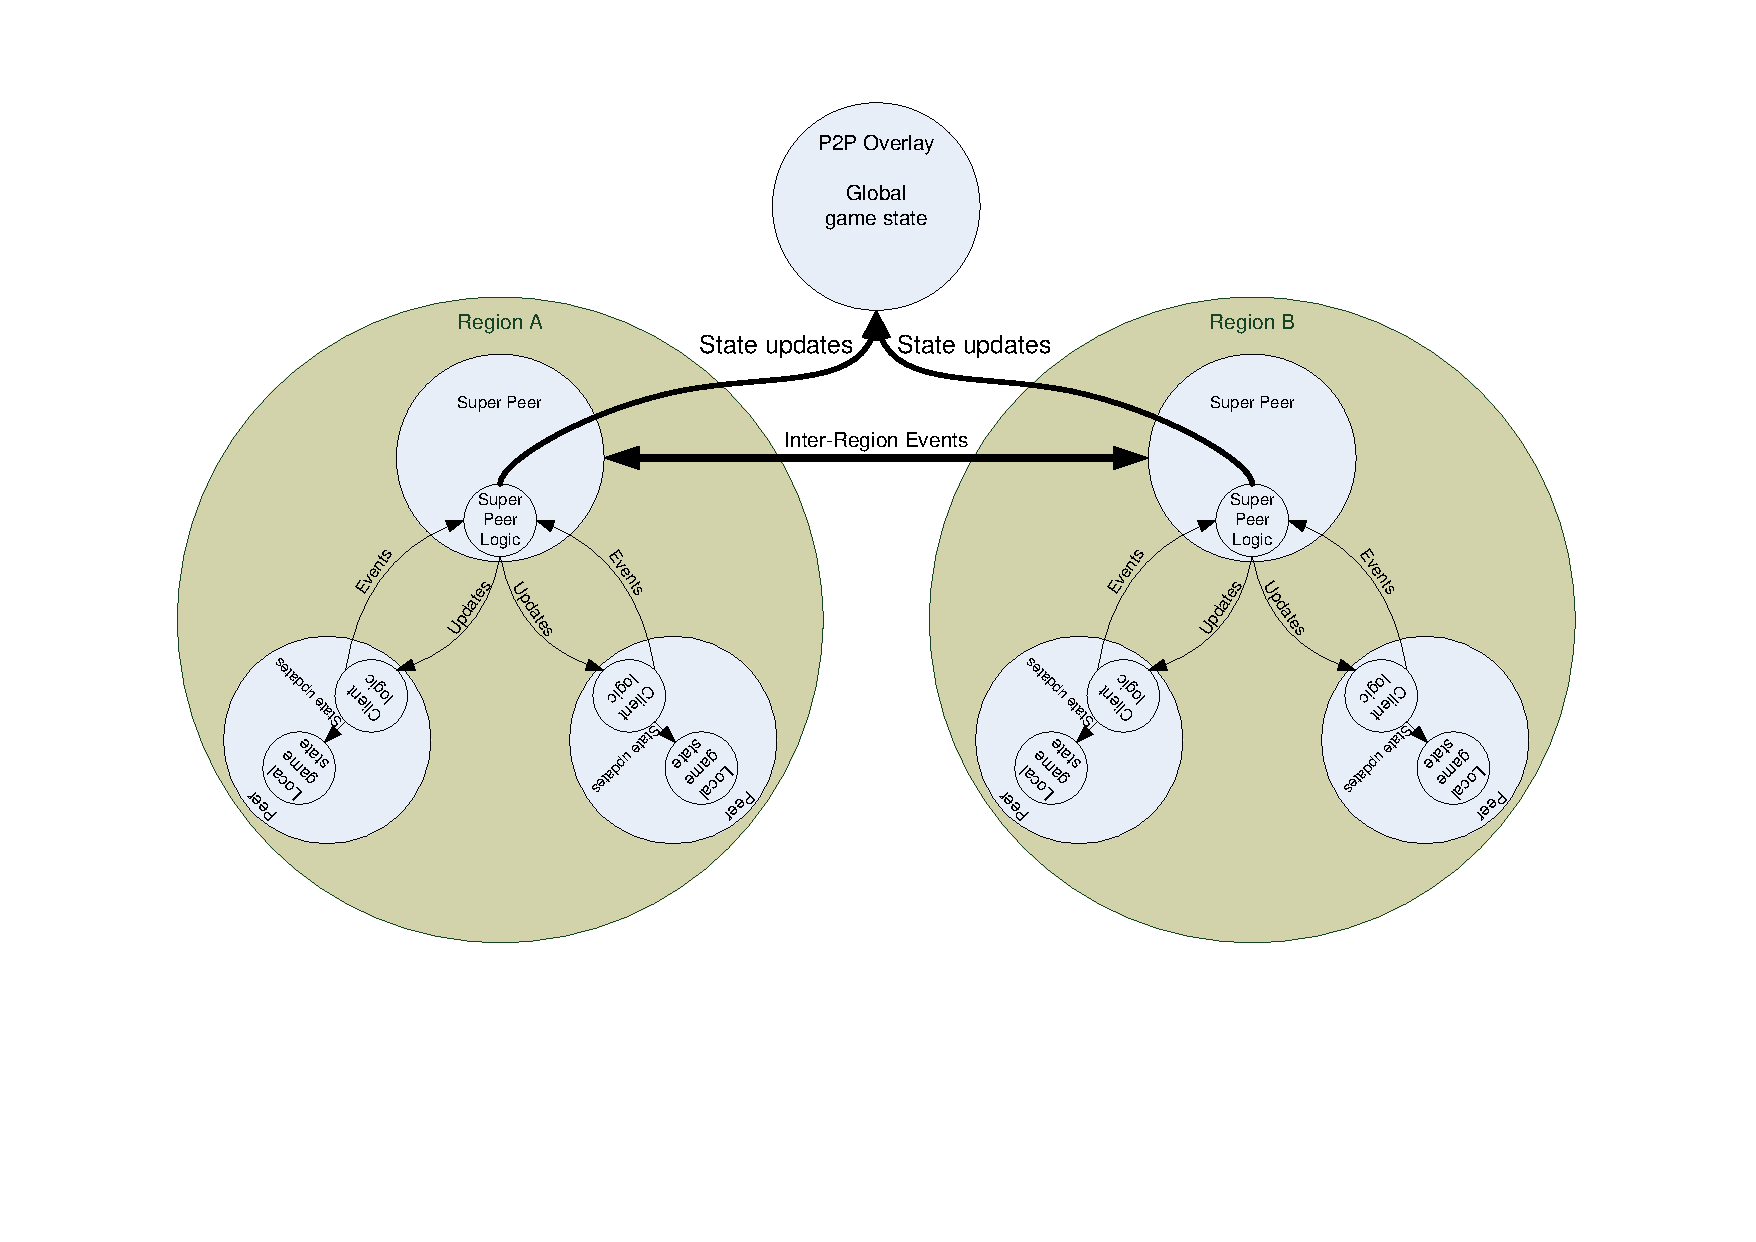
\includegraphics[clip=true, viewport=2cm 5cm 27cm 19.5cm, width=\columnwidth]{region_based_CS_CM_P2PO}
 \caption{Region-based Client/Server with overlay consistency model}
 \label{fig_cs_region_o_cm}
\end{figure}
%
Overlay storage, shown in Figure \ref{fig_cs_region_cm} entails using a distributed file storage system, based on a P2P overlay to host objects. Figure \ref{fig_cs_region_cm} actually shows a type of Super Peer/Overlay hybrid storage implemented in \cite{zoned_federation}, but the basic principles remain the same. The model depicted in Figure \ref{fig_cs_region_cm}, uses an overlay storage managed by regional super peers. The reason for this management is to achieve state consistency. If all nodes were allowed to update the global state stored in the overlay, the world would become inconsistent for many. This is because updates take time to be stored and retrieved and because it can be expected that many nodes will want to access the same stored data when in the same area, the regioning approach again provides a method to achieve synchronisation.

The world is divided into regions and so data stored for one region will have no effect on the sate of other regions. This can of course be debated, but for global specific data a global ``region'' can be created. Super peers then act as servers that use their section of the overlay as their own storage databases. Data consistency may be assured as all access to a region's data is controlled by that region's super peer. The Zoned Federation model further uses local caching at super peers to achieve real-time access to data. Overlay storage is used as a backup mechanism to achieve data persistency and redundancy.

%Overlay storage - reason
Overlay storage is a very popular storage method, currently used by most P2P MMOG architectures. This is believed to be more as a consequence of the use of Scribe than any inherit benefit to P2P MMOGs \cite{past_storage_focus}. This is also the motivation used in Chapter 4 of \cite{Fan_phd}, where the Mediator architecture is described. Scribe is an implementation of \ac{alm} that uses the Pastry overlay as the structure to send multicast messages over \cite{scribe}. PAST is a distributed persistent storage implemented to use Pastry for routing data and requests for data. The reason for using overlay storage in so many implementations seem to be merely the availability after using Scribe. The implementation of state persistency, however, does not have to be linked with the event dissemination scheme. A P2P overlay may be used for event dissemination, and another method can be used to ensure state persistency.

%Overlay storage - issues
An evaluation of overlay storage also shows some issues when used for state persistency in MMOGs. The main issue with this mode of storage is summed up by the creators of PAST: ``Finally, PAST is intended as an archival storage and content distribution utility and not as a general-purpose filesystem. It is assumed that users interact primarily with a conventional filesystem, which acts as a local cache for files stored in PAST.'' \cite{storage_and_chaching_PAST}. This is not how the file system interaction occurs in MMOGs. For responsive MMOGs, a distributed file system is required that allows for real-time file storage and retrieval.

The most significant issue with overlay storage is the delay incurred when storing and retrieving data. As data can be stored anywhere on the network and the network is not fully connected, it takes $O(\log_{2^b}(N))$ hops on average to retrieve or store a data item using Pastry, where $b$ us usually chosen as 4 \cite{storage_and_chaching_PAST}. Although this is a good order complexity for a routing algorithm in a large network, it is not sufficient to support a real-time application.

Different types of overlays have other different advantages and disadvantages. A pure overlay-based storage scheme performs very badly. The scheme is inconsistent, because there is no way to synchronise the order of events amongst nodes, which leads to inconsistent states. This model does have better security than the super peer storage model as data are distributed amongst all peers and redundancy and quorum techniques can be implemented to ensure that files are retrieved with a high level of security. Why the security is rated as average is not because a real lack of security, but because of the network overhead, which a secure system introduces.

To ensure a secure system, copies of files have to be saved at different locations. If a file is retrieved, all copies must be queried and received. All received copies then have to be compared to ensure that the contents are correct. This introduces significant additional network overhead as well as additional load on nodes to serve as copies of files.

Pure overlay storage is, however, very fair, as all nodes share file data and requests equally. Is is also reliable when adequate redundancy is built into the system.

The hybrid region-based overlay storage contains many improvements over pure overlay storage. It is just as reliable as pure overlay storage, but that is where the similarities end. Because all regional files are cached at super peers, the system is very responsive. The use of super peers also allows for strict event ordering to be implemented, which ensures data consistency. The only two issues are fairness and security, which are the same as for the super peer storage model.

\subsection{Distance-based storage}

%Distance-based - overview
Distance based approaches, such as the Voronoi storage approaches \cite{Buyukkaya_voronoi_state_management}, \cite{Hu_voronoi_IM} and also some more general approaches \cite{colyseus_distance_based}, store object data on the peer closest to the object in the virtual world. Some distance metric is used to determine on which node an object should be stored. For the Voronoi approaches, a node controls and hosts all objects within its Voronoi region. The reasoning is that there is a high probability that the player closest to the object is also the player using the object. Examples of this are where a player is trading or fighting with an NPC. The only problem with this reasoning is that usually multiple nodes are interacting with a single object. The examples of the NPC monster and trader are again relevant. Usually many players interact with a trader NPC and usually players attack monster NPCs in groups.

%Distance-based - issues
Multiple player interaction is, however, not really an issue as others have stated \cite{}, when compared to other state persistency approaches. In the best case, the object being used by a player is also hosted on that player's node. If another player requires use of a remotely hosted object, that player may still interact with the object, where the host node is now acting as a server to that player. This means that every player hosting an object becomes a server for that object. For the case where a player interacts with an object hosted locally, there is no object latency. In the case where a player accesses a remotely hosted object, there is only one hop latency, the same as with a client server application. The advantage however is that the total server load for all objects is distributed amongst all peer, which means that each peer should have to handle much less queries than with the super peer storage approach. This might protect peers from becoming overloaded.

Issues with this approach stem from the fact the players are constantly moving. When players move, the objects in their regions change. Objects, therefore, have to be constantly handed over from one peer to another, which might cause significant network traffic. An object in transit might also delay interaction with that object.

Reliability is also an issue, because of network churn. When nodes leave the network, the objects that they controlled should still be accessible. Redundancy and added overlay storage can be implemented here to ensure reliability.

The main issue with the distance based scheme is security. Nodes that have the most interest in an object also have the most interest to manipulate that object in ways inconsistent with the game rules. When objects are hosted on nodes that have the most interest in them, there will be a strong drive to try and manipulate these objects. Because these modification are all local, it is also not possible to log the alterations and detect cheating. Means by which local objects can be secured have to be found or distance based algorithms with quorum need to be investigated.

\begin{table}[htbp]
\centering
\begin{tabular}{|r|c|c|c|c|c|}
\hline
Storage type & Reliability & Responsiveness & Security & Fairness & Consistency\\
\hline
Region-based Super Peer & Medium & High & Low & Low & High\\
Overlay & High & Low & Medium & High & Low\\
Region-based Super Peer/Overlay & High & High & Low & Low & High\\
Distance-based & Low & High & Low & High & Low\\
\hline
\end{tabular}
\caption{Differences between storage mechanisms}
\label{tab_storage}
\end{table}
%
Table \ref{tab_storage} presents a summary of the above discussion on how current storage systems handle the five key issues identified. From this table it can be seen that no one storage mechanism has fully addressed all the identified issues. What is also shown is that architectures that differentiate between different types of data, are theoretically better suited to the MMOG application. The example of such an architecture is the hybrid architecture, which also seems to fares best, when compared to other storage techniques.



\section{Proposed consistency model}
\label{proposed_consistency}

A novel state persistency architecture is proposed in this work, specifically designed to meet the real-time requirements of P2P MMOGs.

\begin{figure}[htbp]
 \centering
 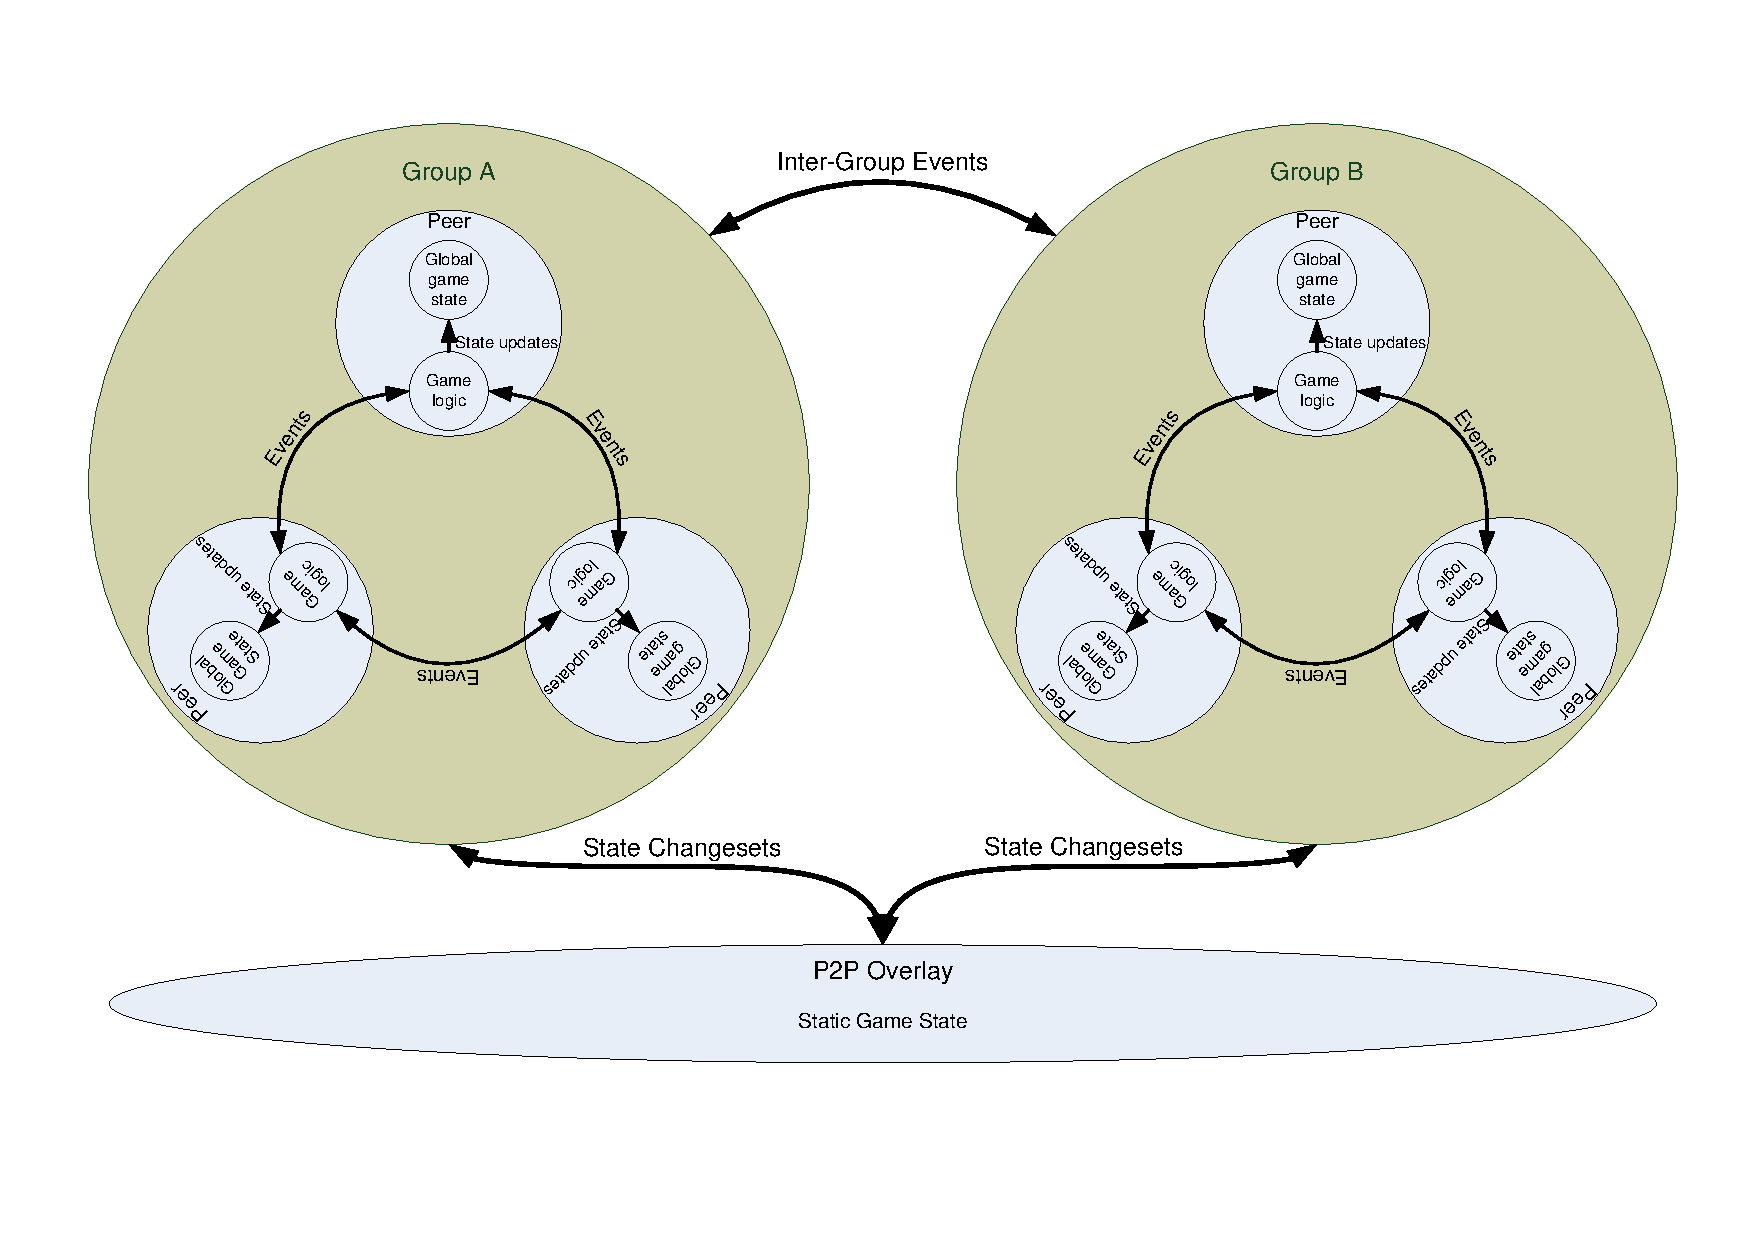
\includegraphics[clip=true, viewport= 1cm 3cm 28.5cm 19cm, width=\columnwidth]{group_based_P2P_P2PO}
 \caption{Group-based Peer-to-Peer with overlay consistency model}
 \label{fig_p2p_group_o_cm}
\end{figure}
%
Figure \ref{fig_p2p_group_o_cm} shows the initial proposed state persistency model for an MMOG. As described in Section \ref{proposed_architecture}, this persistency model is based on groups of players, rather than regions. An architecture is proposed that uses a hybrid model of storage, similar to the Zoned Federation model proposed in \cite{zoned_federation}.

A distinction will be made between ephemeral and permanent data. Where ephemeral data is considered data that is only valid for a short time. An example of this is player movement, which changes frequently, so long term storage is unnecessary. Permanent data are data that remains constant for a significant amount of time. An example if this would be a player attributes or inventory contents.

All players will form part of a specific group. The hierarchical state persistency model on one level operates within groups and on the higher level, amongst groups. The proposal is that ephemeral data will only exist amongst groups with a high level of responsiveness. Unicast connections will be used amongst groups that would enable fast retrieval of ephemeral data such as player position updates. It is also proposed that a fully connected P2P network model is maintained within groups of players. This would allow for high responsiveness.

Ephemeral player data might be stored on a second level overlay storage, which only exist amongst the members of every group. Group data can thus be distributed amongst players to achieve maximum fairness. It is also proposed that no central peer be used to apply game logic to peer events as is the case with super peers.

It should be explored whether an event-based or update-based consistency model should be used within groups. If groups sizes could be bound, the disadvantages named in Section \ref{classic_models} will not be an issue. This would allow for all peers to apply game logic and for validity checking to be done on updates sent from peers. This would increase the security of the system and would prevent any malicious super peer from hijacking the game. How a limited group size will affect the game will be investigated to determine whether it is feasible.

It is then proposed that the overlay acts as a slow, but reliable storage medium. With data being constantly backed up to this medium. If data are lost before it could be backed up, the game should still be able to return to a previously stable state for the players that logged out, after logging back in.

The main purpose of the proposed consistency model is to develop a low latency, highly reliable, consistent, fair and secure storage network. It is proposed that the use of super peers be avoided as much as possible, in order to obtain all benifits of a P2P model.

\section{Related consistency models}
\label{related_cm}

There have been very few papers that deal directly with state persistency in MMOGs. Most papers merely assume that reliable consistent storage is available and sometimes go as far as to propose PAST to be used with Scribe. State persistency has thus far been regarded as a basis to be used to build other MMOG functions on. The few papers that have addresses state persistency directly have been discussed in Section \ref{p2p_mmog_cm}.

The existing model that is nearest to the proposed state persistency model would be the Zoned Federation model \cite{zoned_federation}. The main difference between the Zoned Federation model and the proposed model is that the Zoned Federation model uses super peers for data caching, instead of all nodes in the network. This use of super peers has all the issues of super peer storage, discussed in Section \ref{p2p_mmog_cm}. It is believed that a fair, more secure approach, where all users contribute in accordance with their means, should rather be investigated. That would be the novelty of the proposed persistency model.

\section{Proposed evaluation techniques}
\label{evaluation_techniques}

What became evident while performing the literature study, was that there are no quantitative studies, comparing different P2P MMOG architectures or P2P MMOG architectures to C/S MMOG architectures. The reason for this is believed to be the incompleteness of most P2P MMOG architectures and also the difficulties with a test setup that would compare P2P to C/S.

The difficulties with a test setup that would compare P2P to C/S is that the same application layer data should be compared. In other words, the same game should be used to test both architectures. The reason for this being that different games have implemented different networking architectures, as well as different communications protocols. The sizes and number of packets will differ. Some games may have implemented a more efficient communications protocol with less network overhead. To be able to accurately test the two architectures then, the same communications protocol should execute over these architectures. The main issue with this is that communications protocols differ from C/S to P2P. As each of these architectures have different advantages and disadvantages, communication protocols executing over them will have to implement different mechanisms to cope with each architecture. The security mechanisms, for example, will look very different from one architecture to the other.

In an effort to compare P2P to C/S, a test setup is proposed that would theoretically allow the two architectures to be used for the same game. It is proposed that an existing open source C/S MMOG server be adopted for P2P. Every player will have both a client and server installed on her computer. The existing game client will connect to the modified game server on the same host. The game servers on all hosts will then form a P2P network and function as the P2P MMOG.

This approach will allow for the same game to be compared with the two different architectures, it will also allow for comparison between different P2P architectures if the server alterations are implemented as an extra middleware layer, with which architectures may interact over a standard interface.

The evaluation process will have multiple stages. The first stage will be the theoretical evaluation of the proposed consistency model and the comparison with other models. This will mostly be performed using simulation. Grouping algorithms first have to be investigated on which the consistency model and network architecture will be built.

A consistency model will then be developed using the grouping algorithm. This model will then be tested according to the challenges identified in Section \ref{key_challenges_cm}. A measurable metric will also have to be defined for each of the identified issues. Other consistency models will also be simulated in order to compare their performance with the proposed model. Player movement data is required for this simulation. If possible, real game traces will be obtained and used to test the consistency model performance with actual players movements. If this is not possible, player movement would have to be simulated, which could be become complex as the concept of player flocking should also then be simulated.

After the consistency model has been developed, the test framework for the P2P MMOG architecture will be developed. Existing P2P MMOG architectures will be used to define the interface of the framework. Working architectures will then be compared, using the testing framework to determine how the overall architectures perform. After a performance comparison, a study should be undertaken as to what the performance bottlenecks are. The proposed network architecture will then be developed, using what was learned from the study.

%\section{Expected contributions}
%\label{expected_outcomes}

\section{Conclusion}

This study has three expected outcomes. The main outcome will be a state consistency model that is provably better than currently used models for P2P MMOGs. The second part of the contribution is developing a P2P MMOG architecture, which uses the new state consistency model to achieve better performance than current architectures. The third contribution will be to compare different architectures and consistency models and determine which of the other proposed architectures in the literacy work better with a P2P MMOG.

This proposal presents an extensive literature study into what the state of the art is of P2P MMOGs. The P2P MMOG architecture is compared to more classic architectures, both in terms of the overall network architecture, as well as in terms of the consistency models employed. After a thorough investigation into the issues of P2P MMOG, it was determined that state persistency and consistency are areas that still require much attention. With this in mind a novel networking architecture as well as a consistency model were proposed that hopes to address some of the issues related to P2P MMOGs. Finally, possible testing techniques and a testing framework were presented. The framework will be used to test all contributions and enable a rigourous  

\newpage
\bibliographystyle{IEEEtran}
\bibliography{P2P_MMOG}

% that's all folks
\end{document}


